\documentclass[preprint,12pt]{elsarticle}
\usepackage{lmodern}
\usepackage{amsmath,amssymb}
\usepackage{graphicx}
\usepackage{booktabs}
\usepackage{multirow}
\usepackage{array}
\usepackage{xcolor}
\usepackage[section]{placeins}
\usepackage{float}
\usepackage{xr-hyper}
\usepackage{hyperref}
\externaldocument[S-]{supplementary}
\hypersetup{hidelinks,
  pdftitle={CanonFuse3D: Reliability-Gated Fusion of Uncalibrated Dual-View 3D Human Pose Streams for Fast-Moving Athletes},
  pdfauthor={Kaixu Chen, Qingyu Wang, Chun Xie, Eiichi Naito, Toshitaka Kimura, Itaru Kitahara}}
\usepackage{lineno}
\setlength{\emergencystretch}{2em}
\journal{Image and Vision Computing}

% Upright prose, including class-generated headings and bibliography emphasis.
\AddToHook{begindocument/end}{%
  \renewcommand{\itshape}{\fontshape{n}\selectfont}%
  \renewcommand{\slshape}{\fontshape{n}\selectfont}%
}
\renewcommand{\textit}[1]{\textup{#1}}
\renewcommand{\emph}[1]{\textup{#1}}

\begin{document}

\begin{frontmatter}

\title{CanonFuse3D: Reliability-Gated Fusion of Uncalibrated Dual-View 3D Human Pose Streams for Fast-Moving Athletes}

\author[ccs]{Kaixu Chen\corref{cor1}}
\ead{chenkaixusan@gmail.com}
\author[imiss]{Qingyu Wang}
\ead{wang.qingyu@image.iit.tsukuba.ac.jp}
\author[ccs]{Chun Xie}
\ead{xie.chun@image.iit.tsukuba.ac.jp}
\author[nict]{Eiichi Naito}
\ead{eiichi.naito@nict.go.jp}
\author[ntt]{Toshitaka Kimura}
\ead{toshitaka.kimura@ntt.com}
\author[ccs]{Itaru Kitahara}
\ead{kitahara.itaru@image.iit.tsukuba.ac.jp}

\cortext[cor1]{Corresponding author.}
\address[ccs]{Center for Computational Sciences, University of Tsukuba, 1-1-1 Tennodai, Tsukuba, Ibaraki 305-8577, Japan}
\address[imiss]{Degree Programs in Systems and Information Engineering, Graduate School of Science and Technology, University of Tsukuba, 1-1-1 Tennodai, Tsukuba, Ibaraki 305-8573, Japan}
% CONFIRM with E. Naito: CiNet is the Advanced ICT Research Institute unit at Yamadaoka; adjust if his affiliation is worded differently.
\address[nict]{Center for Information and Neural Networks (CiNet), Advanced ICT Research Institute, National Institute of Information and Communications Technology, 1-4 Yamadaoka, Suita, Osaka 565-0871, Japan}
% CONFIRM with T. Kimura: NTT CS Labs headquarters is Atsugi (previously written as Tokyo).
\address[ntt]{NTT Communication Science Laboratories, NTT, Inc., 3-1 Morinosato-Wakamiya, Atsugi, Kanagawa 243-0198, Japan}

\begin{abstract}
Monocular three-dimensional (3D) human pose estimates remain vulnerable to depth ambiguity, self-occlusion, and temporal jitter. A second camera can provide complementary evidence, but exploiting it through calibrated reconstruction is difficult when cameras follow a distant, fast-moving athlete or are installed temporarily. We present CanonFuse3D, a calibration-free post-estimation framework that fuses two independently estimated, approximately synchronized monocular 3D pose streams without requiring images, 2D observations, or camera parameters at the fusion stage. Human-centric canonicalization and sequence-level alignment expose cross-view agreement and disagreement; a shared joint encoder, bidirectional cross-view attention, and temporal refinement then drive joint-frame gating with residual correction. We evaluate the framework quantitatively on a synthetic Unity dataset with avatar ground truth and the real-world Ski-PTZ-Pose dataset with a constructed reference, and qualitatively on author-collected dual-view recordings. Relative to canonical averaging, CanonFuse3D reduces the mean per-joint position error by 44.5\% on Unity and 48.6\% on Ski-PTZ-Pose, while comparisons with learned and geometric references reveal metric- and input-dependent trade-offs rather than universal superiority. Controlled studies characterize the useful range across camera separations, small timing and sampling-rate errors, and pose or image occlusion, including failures under severe corruption. The same architecture supports alternative pose estimators through lightweight adaptation and additional cameras through pairwise composition.
\end{abstract}

\begin{keyword}
3D human pose estimation \sep dual-view fusion \sep post-estimation pose fusion \sep calibration-free refinement \sep human-centric representation \sep front-end generalization
\end{keyword}

\end{frontmatter}

\linenumbers

\section{Introduction}

Monocular three-dimensional (3D) human pose estimation spans temporal lifting of 2D keypoints~\cite{pavllo2019videopose3d,zheng2021poseformer,li2022mhformer}, pretrained motion representations~\cite{zhu2023motionbert}, video-based body models~\cite{kocabas2020vibe}, and foundation-scale full-body estimators~\cite{yang2026sam}. These methods support sports motion analysis, but their outputs retain depth ambiguity, self-occlusion, viewpoint-dependent errors, and temporal jitter. Skiing combines rapid movement, distant observation, and continuous orientation changes, making these limitations particularly relevant~\cite{rhodin2018learning,chen2021sportscap}. Complementary viewpoints can reveal a limb hidden in one camera and provide depth estimates with different errors.

Exploiting a second view usually requires information beyond the two monocular outputs. Binocular methods use stereo keypoints or jointly refine 2D and 3D poses through geometric constraints~\cite{wan2025rsb,wan2024dualdiffusion}; calibrated multi-view methods triangulate detections or exchange image features under known geometry~\cite{iskakov2019learnable,he2020epipolar,liao2024multiple,zhang2021adafuse}. Temporary placement and pan--tilt--zoom operation make calibration harder to maintain in skiing. Unknown-calibration methods relax that requirement: MetaPose initializes from monocular 3D estimates but retains 2D evidence when refining pose and camera variables~\cite{usman2022metapose}. The relevant distinction is therefore what information cross-view refinement requires, rather than whether it reuses a monocular estimator.

We study post-estimation fusion when only two independently predicted, approximately synchronized 3D sequences on a common joint set are available to the fusion stage. The objective is a more accurate and temporally stable canonical sequence without supplying that stage with images, 2D detections, intrinsics, or extrinsics. These restrictions do not apply to the upstream estimators that process RGB frames. The output is human-centric rather than a recovered world-coordinate trajectory, and additional cameras are considered separately through pairwise composition. This interface allows an existing monocular pipeline to incorporate complementary predictions without introducing calibrated image-space reconstruction.

CanonFuse3D~\cite{chen2026canonfuse3dconference} (Figure~\ref{fig:teaser}) canonicalizes the streams using body landmarks and aligns them by sequence-level similarity transforms. Features describing pose agreement, disagreement, motion, and alignment feed a shared encoder, bidirectional cross-view attention, and temporal refinement. A joint-frame gate combines view-specific candidates with a learned residual correction. This article builds on the architecture of~\cite{chen2026canonfuse3dconference} and focuses on its robustness, front-end generalization, and extension to additional views. Keeping the upstream estimator separate allows the architecture to accept alternative estimators on the common joint set, although transfer of trained fusion weights requires experimental validation.

\begin{figure}[t]
  \centering
  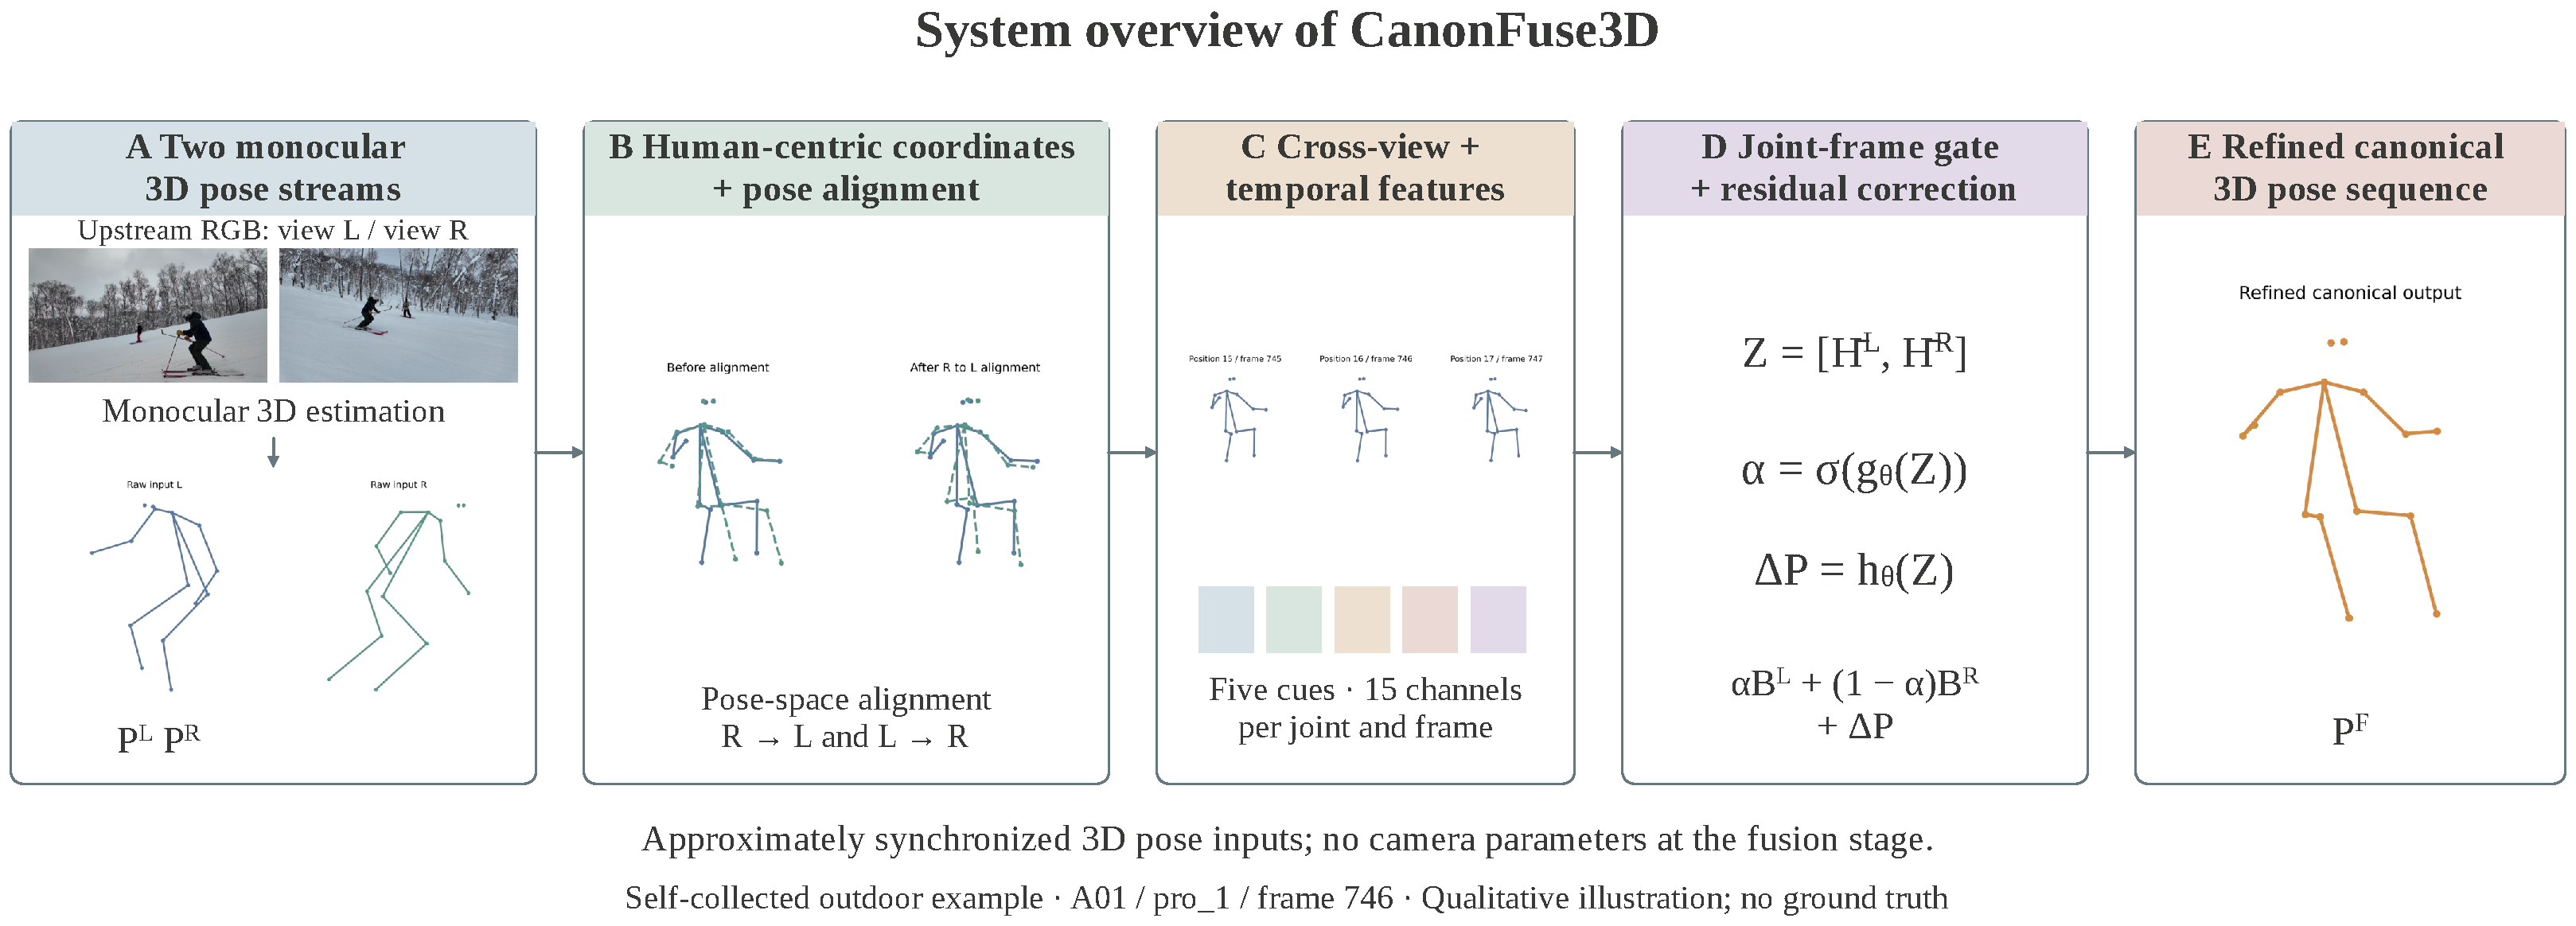
\includegraphics[width=\linewidth]{figures/journal/study_overview_visio.pdf}
  \caption{System overview of CanonFuse3D. (A) Two monocular 3D pose streams are estimated independently; (B) they are expressed in human-centric coordinates and aligned in pose space; (C) cross-view and temporal features are built from five cues; (D) a joint-frame gate and residual head fuse the two candidates; (E) a refined canonical 3D sequence is output. No camera parameters are used. The frames are a qualitative author-collected example.}
  \label{fig:teaser}
\end{figure}

We evaluate the framework on three skiing datasets: a synthetic Unity dataset with avatar ground truth, the public Ski-PTZ-Pose dataset with a constructed canonical reference, and author-collected indoor and outdoor recordings used for qualitative deployment. Beyond clean-input accuracy, controlled studies examine how the same model behaves when the camera separation, timing, or sampling rate changes, when pose evidence or image regions are missing, when the upstream estimator is replaced, and when more than two cameras are available.

The main contributions are:
\begin{itemize}
    \item A complete formulation of the human-centric fusion framework for calibration-free post-estimation dual-view 3D pose fusion, including its coordinate conventions, sequence-level alignment, and training objective, together with a controlled ablation of its reliability gate and residual correction.
    \item Quantitative evaluation on two skiing datasets with explicit reference regimes, separating canonical-space comparisons from an independent native-output audit and distinguishing pose-only baselines, published-method adaptations, and additional-input geometric references, complemented by qualitative deployment examples.
    \item A systematic robustness analysis covering camera separation, timing and sampling-rate errors, and both pose-level and image-level occlusion, which identifies the useful operating range and its failure cases.
\end{itemize}

\section{Related Work}
\label{sec:related_work}

\subsection{Monocular 3D Human Pose Estimation}
Two-stage pipelines lift detected 2D trajectories to 3D using temporal convolutions (VideoPose3D~\cite{pavllo2019videopose3d}), spatial--temporal transformers (PoseFormer~\cite{zheng2021poseformer}), multiple hypotheses (MHFormer~\cite{li2022mhformer}), or pretrained motion representations (MotionBERT~\cite{zhu2023motionbert}). Separating lifting from detection permits matched-track comparisons, as in our alternative-front-end study, but errors in the 2D observations still propagate to 3D. The shared keypoint interface does not make the recovered streams interchangeable: estimator-specific limb bias and temporal statistics can remain after coordinate alignment. Our controlled comparison therefore distinguishes the architecture's ability to accept a front end from the transferability of its trained weights.

Visual body estimators operate directly on images or video. SAM 3D Body recovers body, hand, and foot pose and shape from an image~\cite{yang2026sam}, while VIBE combines video features with an adversarial motion prior~\cite{kocabas2020vibe}. Both can supply pose streams to a downstream refinement stage. Keeping that stage separate avoids replacing the upstream estimator, but also limits refinement to information retained in its predicted poses.

Sports impose additional distribution shifts through rapid, atypical motion and self-occlusion. Rhodin et al. introduced Ski-Pose PTZ-Camera and used multi-view consistency to supervise monocular prediction~\cite{rhodin2018learning}; SportsCap instead uses sub-motion priors for monocular sports videos~\cite{chen2021sportscap}. Both remain monocular at inference. Our setting assumes two simultaneously available streams and studies how their potentially different errors can be reconciled after estimation.

\subsection{Dual-view and Multi-view 3D Pose Estimation}
Binocular methods exploit geometric redundancy within reconstruction. RSB-Pose estimates stereo keypoints with disparity-indexed features and refines poses with a pretrained transformer~\cite{wan2025rsb}. Dual-Diffusion jointly denoises binocular 2D and 3D poses using geometry and baseline-dependent normalization~\cite{wan2024dualdiffusion}. Their image/2D and stereo-geometry interfaces differ from refinement supplied only with predicted 3D streams.

Markerless multi-view estimation faces continuing challenges in occlusion, camera variation, supervision, temporal consistency, view selection, and computational cost~\cite{nogueira2025survey}. Learnable Triangulation combines views through differentiable algebraic or volumetric triangulation~\cite{iskakov2019learnable}. Epipolar Transformers transfer image features along calibrated epipolar lines~\cite{he2020epipolar}, while MVGFormer alternates appearance processing with geometric triangulation of refined 2D poses~\cite{liao2024multiple}. AdaFuse estimates heatmap correspondences and camera-specific weights to limit unreliable-view contributions~\cite{zhang2021adafuse}. These methods reconcile observations inside an image-, feature-, or geometry-based estimator.

MetaPose is closer to post-estimation fusion: it initializes pose and camera variables from monocular 3D predictions, then refines them with a learned optimizer and 2D uncertainty, without supplied calibration or multi-view 3D supervision~\cite{usman2022metapose}. Its 2D and projection terms remain additional inputs in our labeled two-view adaptation. FLEX predicts view-invariant skeletal rotations and bone lengths from multiple streams without supplied extrinsics~\cite{gordon2022flex}. Applying general multi-view methods to two cameras does not remove their observation requirements. Our distinction is the restricted 3D-only interface, not the invention of two-view fusion. Accordingly, calibration-free methods should be compared by their required observations and recovered representation, rather than grouped solely by whether external camera parameters are supplied. The benchmark retains these distinctions instead of presenting additional-input methods as identical-interface replacements.

Takahashi et al.~\cite{takahashi2018human} use detected 2D joints to jointly estimate extrinsics, temporal offsets, and 3D poses from unsynchronized, uncalibrated cameras. CanonFuse3D instead assumes approximate synchronization and measures its residual timing tolerance experimentally.

\subsection{Pose-Space Refinement, Reliability, and Generalization}
STRIDE fits a motion prior to each video through model-agnostic test-time training, refining noisy 3D estimates under occlusion~\cite{lal2025stride}. Its focus is temporal refinement of one video rather than reconciliation of synchronized views. Reliability weighting also operates within Learnable Triangulation and AdaFuse~\cite{iskakov2019learnable,zhang2021adafuse}. Here the gate acts after monocular estimation, weighting aligned 3D candidates at the joint--frame level. Upstream confidence, feature quality, and residual pose-space reliability are therefore distinct signals. A confidence score attached to an image observation does not directly characterize disagreement after pose alignment, and the learned gate must be evaluated against its actual candidates rather than interpreted as a raw-camera confidence.

Distribution adaptation addresses another deployment boundary. PoseAug differentiably varies posture, body size, viewpoint, and position to augment paired 2D--3D training poses~\cite{gong2021poseaug}. AdaptPose generates target-like motions and cameras using target-domain 2D poses without target 3D labels or camera information~\cite{gholami2022adaptpose}. Both adapt a pose estimator's training distribution. Our experiments instead keep the fusion architecture fixed, replace its upstream estimator, and compare frozen transfer with front-end-specific or mixed adaptation. The evaluation thus tests both the benefit of complementary 3D predictions and the conditions under which that benefit fails.

\section{Proposed Method}
\label{sec:method}

\subsection{Overview}
\label{subsec:method_overview}

CanonFuse3D~\cite{chen2026canonfuse3dconference} maps two independently estimated, approximately synchronized pose sequences \(P^L,P^R\in\mathbb{R}^{T\times J\times3}\) to a canonical sequence \(P^F\) of the same shape, where \(T\) and \(J\) denote frames and joints. Images and 2D observations remain upstream; the fusion module neither receives camera parameters nor reconstructs a world-coordinate trajectory. Figure~\ref{fig:feature_construction} groups the pipeline into canonicalization and alignment (stages 1--3), five-cue feature construction (stage 4), and cross-view temporal refinement with gated residual fusion (stages 5--8).

\begin{figure}[!t]
  \centering
  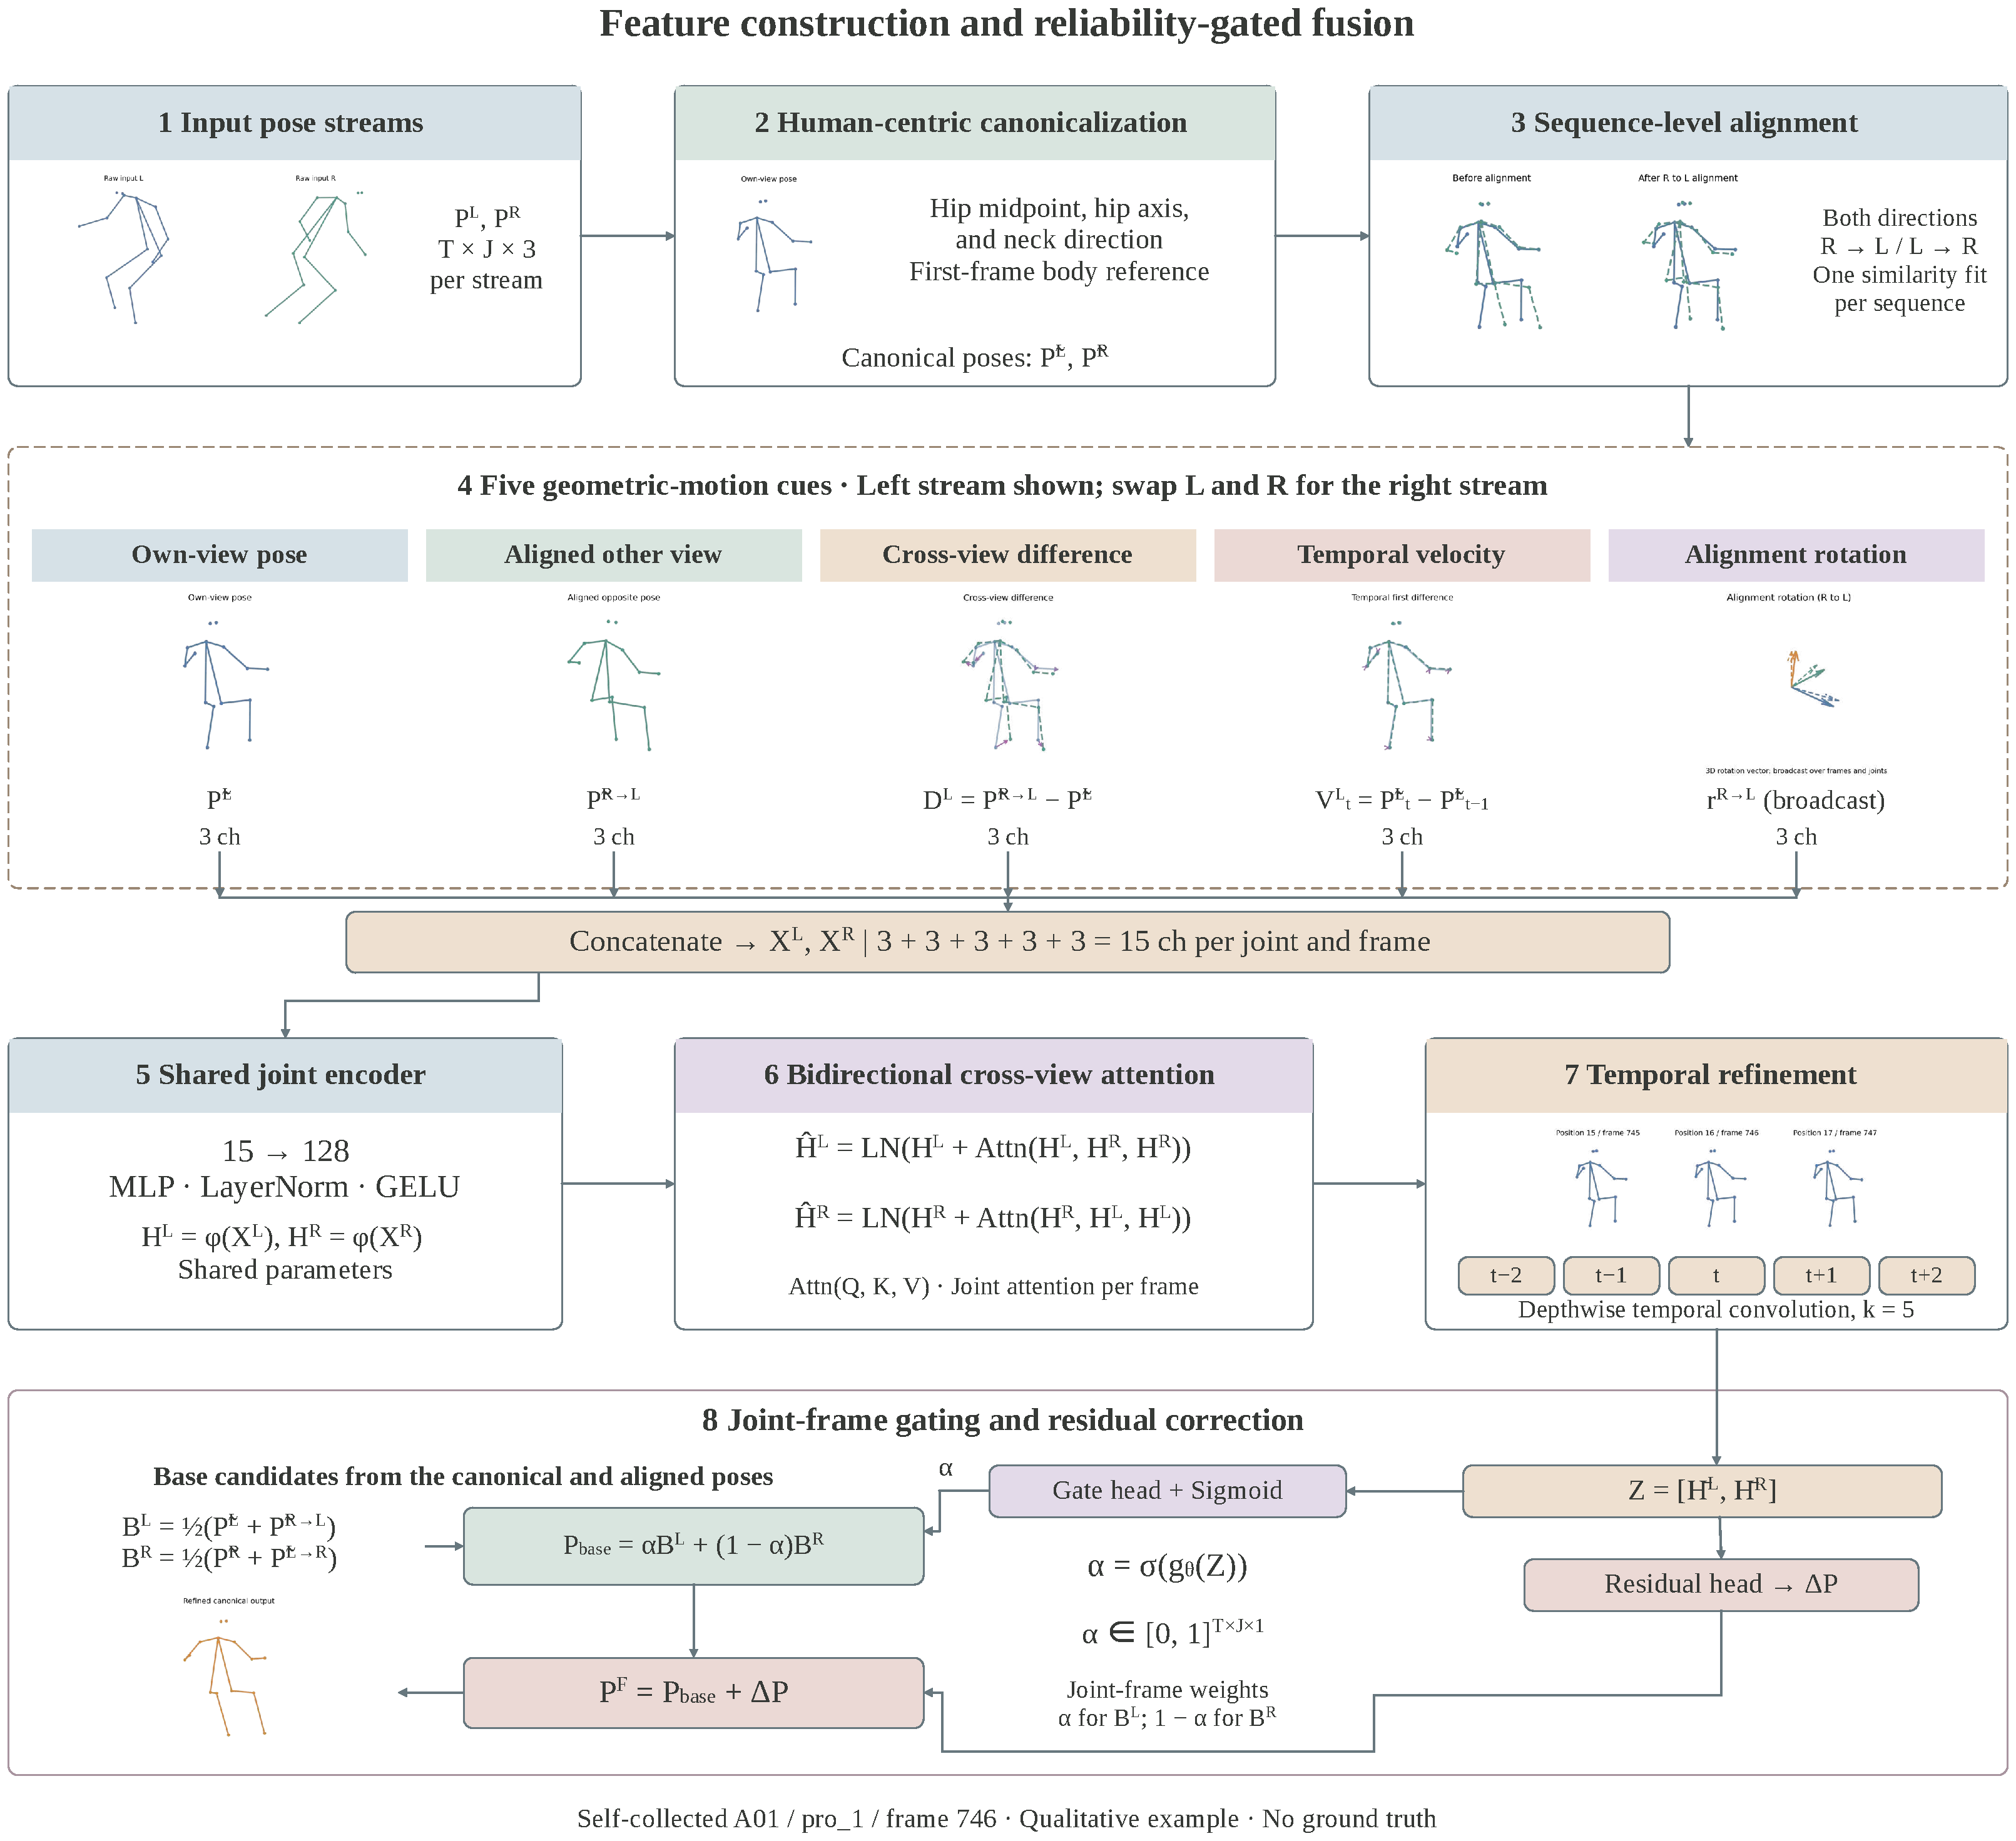
\includegraphics[width=\linewidth]{figures/journal/method_pipeline_visio.pdf}
  \caption{CanonFuse3D pipeline. Stages 1--3 canonicalize and align the two streams; stage 4 concatenates five three-dimensional cues into a 15-channel feature per joint and frame; stages 5--8 encode the features, apply cross-view attention and temporal refinement, and fuse the base candidates \(B^L\) and \(B^R\) through the gate \(\alpha\) with residual \(\Delta P\). The right stream swaps the view roles.}
  \label{fig:feature_construction}
\end{figure}

\subsection{Human-Centric Landmark Canonicalization}
\label{subsec:canonicalization}

Independent monocular estimates can differ in global position and orientation. We express each stream relative to a fixed reference pose \(A\) using the hip midpoint, hip direction, and neck direction. Let \(h_L,h_R,n\) denote the left hip, right hip, and neck, and let \(\operatorname{nrm}(v)=v/(\|v\|_2+\epsilon)\). The origin and body axes are
\[
\begin{aligned}
c&=\tfrac12(A_{h_L}+A_{h_R}), &
e_x&=\operatorname{nrm}(A_{h_R}-A_{h_L}),\\
e_y&=\operatorname{nrm}(A_n-c), &
e_z&=\operatorname{nrm}(e_x\times e_y).
\end{aligned}
\]
An additional landmark-direction cue resolves the sign of \(e_z\). With the axis matrix \(R=[e_x,e_y,e_z]\), the transformed coordinates are
\[
\tilde{P}_{t,j}=(P_{t,j}-c)R.
\]
The left stream, right stream, and supervision reference use separate body references. Each origin and axis matrix remains fixed over the sequences to which it is applied; the representation is therefore not a per-frame root-relative pose. Skeleton scale is not normalized, and the constructed axes need not be orthogonal. In the evaluated protocol, the reference is shared within each batch. Its exact selection and landmark conventions are specified in Supplementary Section~\ref{S-sec:implementation_record}.

\subsection{Pose-Level Cross-View Alignment}
\label{subsec:pose_alignment}

To reduce residual translation, orientation, and scale mismatch, we align each anchored stream to the other:
\[
\tilde{P}^{L \rightarrow R} = \mathcal{A}(\tilde{P}^{L}, \tilde{P}^{R}),
\qquad
\tilde{P}^{R \rightarrow L} = \mathcal{A}(\tilde{P}^{R}, \tilde{P}^{L}),
\]
where \(\mathcal{A}\) estimates a sequence-level similarity transform.

For each sample, let \(X,Y\in\mathbb{R}^{N\times3}\) contain the source and destination joint coordinates in row-vector form, with \(N=TJ\). We estimate one uniform scale \(s\), proper rotation \(Q\), and translation \(d\) for the whole sequence:
\[
(s^\star,Q^\star,d^\star)=
\underset{s\geq0,\;Q\in SO(3),\;d\in\mathbb{R}^{3}}{\arg\min}
\frac{1}{N}\left\|sXQ^\top+\mathbf{1}d^\top-Y\right\|_F^2.
\]
We solve this unweighted least-squares problem by singular value decomposition with the proper-rotation correction of Umeyama~\cite{umeyama1991least}, excluding reflections. Each direction uses one transform for all frames and joints in the sequence. These auxiliary pose-space transforms do not estimate camera extrinsics; they are also distinct from the per-frame reference alignment used only for evaluation.

The model requires dense, finite pose tensors and receives no joint-validity mask. Missing detections are represented by zero-filled raw poses, and the controlled pose-corruption study replaces or perturbs selected raw entries before canonicalization. All transformed entries participate equally in alignment and training, including corrupted or zero-filled entries; missing joints are neither interpolated nor omitted. Detection-failure flags are used only for reporting, and supervision references remain uncorrupted. Supplementary Section~\ref{S-sec:controlled_details} gives the intervention rules.

We further compute cross-view residuals:
\[
D^{L} = \tilde{P}^{R \rightarrow L} - \tilde{P}^{L},
\qquad
D^{R} = \tilde{P}^{L \rightarrow R} - \tilde{P}^{R}.
\]
These residuals encode disagreement between the two pose streams and provide cues about view-specific errors.

\subsection{Geometric-Motion Feature Construction}
\label{subsec:feature_construction}

Stage 4 of Figure~\ref{fig:feature_construction} concatenates five three-dimensional cues at every joint and frame:
\[
\begin{aligned}
X^{L}&=[\tilde{P}^{L},\tilde{P}^{R \rightarrow L},D^{L},V^{L},r^{R \rightarrow L}],\\
X^{R}&=[\tilde{P}^{R},\tilde{P}^{L \rightarrow R},D^{R},V^{R},r^{L \rightarrow R}].
\end{aligned}
\]
Velocity is the first temporal difference, \(V^{L}_{t}=\tilde{P}^{L}_{t}-\tilde{P}^{L}_{t-1}\) with \(V^{L}_{1}=0\), and likewise for \(V^R\). Each alignment rotation vector \(r\) is broadcast across all joints and frames. The resulting 15-dimensional feature describes the own-view estimate, aligned opposite estimate, disagreement, local motion, and sequence-level rotation. The two pose cues expose alternative configurations in one stream's pose space, while their residual measures disagreement explicitly. Velocity supplies local motion context, and the broadcast rotation describes the global relation between streams. These cues inform candidate reliability; they are feature components, not separately trained prediction branches.

\subsection{Joint Feature Encoding}
\label{subsec:joint_feature_encoding}

A shared joint-wise encoder maps the 15-dimensional features to 128-dimensional hidden representations:
\[
H^{L} = \phi(X^{L}),\qquad H^{R} = \phi(X^{R}).
\]
The encoder \(\phi\) is a two-layer multilayer perceptron, each layer followed by layer normalization and GELU activation, preserving the joint and frame indices. Weight sharing applies the same feature mapping to both views. Cross-view exchange occurs in the following attention stage rather than inside this joint-wise encoder.

\subsection{Bidirectional Cross-View Attention}
\label{subsec:cross_view_attention}

Within each frame, each view attends to the other view's \(J\) joint features:
\[
\begin{aligned}
\hat{H}^{L}&=\mathrm{LN}\!\left(H^{L}+\mathrm{Attn}(Q=H^{L},K=H^{R},V=H^{R})\right),\\
\hat{H}^{R}&=\mathrm{LN}\!\left(H^{R}+\mathrm{Attn}(Q=H^{R},K=H^{L},V=H^{L})\right).
\end{aligned}
\]
The two multi-head attention directions have separate parameters. Residual connections and layer normalization retain the own-view features while incorporating cross-view evidence. Attention spans joints within a frame, allowing both corresponding and related joints to contribute. Temporal interaction is handled by the next module.

\subsection{Temporal Refinement}
\label{subsec:temporal_refinement}

For each joint, temporal refinement applies layer normalization, a depthwise one-dimensional convolution of kernel size 5, GELU, dropout, and a pointwise convolution:
\[
\bar{H} = \hat{H} + \mathrm{TempConv}(\mathrm{LN}(\hat{H})).
\]
The same module processes both streams, adding short-range motion context to their cross-view features. Its residual path preserves the input representation while learning a local correction. This temporal feature update precedes the gate and is distinct from smoothing the final output poses.

\subsection{Reliability-Gated Fusion and Residual Correction}
\label{subsec:reliability_fusion}

Concatenated features drive two two-layer perceptron heads with GELU activation:
\[
Z=[\bar{H}^{L},\bar{H}^{R}],\qquad
\alpha=\sigma(g_{\theta}(Z)),\qquad
\Delta P=h_{\theta}(Z).
\]
Here \(\sigma\) is logistic and \(\alpha\in[0,1]^{T\times J\times1}\) weights two view-specific pose candidates:
\[
\begin{aligned}
B^{L}&=\tfrac12(\tilde{P}^{L}+\tilde{P}^{R\rightarrow L}),&
B^{R}&=\tfrac12(\tilde{P}^{R}+\tilde{P}^{L\rightarrow R}),\\
P^{base}&=\alpha B^{L}+(1-\alpha)B^{R},&
P^{F}&=P^{base}+\Delta P.
\end{aligned}
\]
Because the streams have separate body references, this learned pose-space combination does not imply a shared physical frame. The gate is a learned reliability signal, not calibrated probabilistic uncertainty.

\subsection{Training Objective}
\label{subsec:training_objective}

The model is trained with a supervised pose loss and four lightweight regularization terms:
\[
\mathcal{L}
=
\mathcal{L}_{sup}
+
\lambda_{view}\mathcal{L}_{view}
+
\lambda_{bal}\mathcal{L}_{bal}
+
\lambda_{ent}\mathcal{L}_{ent}
+
\lambda_{temp}\mathcal{L}_{temp}.
\]
The supervised term is the mean absolute error to the independently canonicalized reference \(\tilde{G}\),
\[
\mathcal{L}_{sup}=\frac{1}{3TJ}\sum_{t,j}\|P^{F}_{t,j}-\tilde{G}_{t,j}\|_{1}.
\]
The view-reconstruction term preserves the discrepancy between the two canonicalized inputs. With \(\delta=\tilde{P}^{L}-\tilde{P}^{R}\), the fused pose and gate reconstruct the two inputs as \(\hat{P}^{L}=P^{F}+(1-\alpha)\delta\) and \(\hat{P}^{R}=P^{F}-\alpha\delta\), and
\[
\mathcal{L}_{view}=\frac{1}{2}\left(\frac{1}{3TJ}\sum_{t,j}\|\hat{P}^{L}_{t,j}-\tilde{P}^{L}_{t,j}\|_{1}
+\frac{1}{3TJ}\sum_{t,j}\|\hat{P}^{R}_{t,j}-\tilde{P}^{R}_{t,j}\|_{1}\right).
\]
This term constrains the gate and fused estimate without treating the sequence-level similarity transforms as physical camera geometry. Two gate penalties avoid degenerate fusion: the balance term \(\mathcal{L}_{bal}=|\bar{\alpha}-0.5|\), where \(\bar{\alpha}\) is the mean gate over all joints and frames, discourages collapse to a single view, and the negative-entropy term
\[
\mathcal{L}_{ent}=\frac{1}{TJ}\sum_{t,j}\left[\alpha_{t,j}\log\alpha_{t,j}+(1-\alpha_{t,j})\log(1-\alpha_{t,j})\right]
\]
discourages overconfident gates during training. Finally, the temporal term penalizes second-order variation of the fused trajectory,
\[
\mathcal{L}_{temp}=\frac{1}{(T-2)J}\sum_{t=2}^{T-1}\sum_{j}\|P^{F}_{t+1,j}-2P^{F}_{t,j}+P^{F}_{t-1,j}\|_{2},
\]
encouraging stable motion without removing the supervised accuracy objective. The weights are \(\lambda_{view}=0.05\), \(\lambda_{bal}=0.02\), \(\lambda_{ent}=0.005\), and \(\lambda_{temp}=0.01\). All sums are additionally averaged over the mini-batch. No term uses an input-visibility mask to omit or reweight missing joints: an available reference still supervises the output at every joint, while a zero-filled input remains part of the view-reconstruction target.

\section{Experimental Protocol}

\subsection{Experimental Setup}

Upstream estimators process the views independently. CanonFuse3D and pose-only controls receive their 3D sequences; geometric controls additionally receive estimated 2D joints and supplied calibration. Within each dataset and coordinate protocol, comparisons use matched sequences and joint conventions.

\subsection{Data Sources and Annotation}
\label{subsec:dataset_annotation}

We use three skiing datasets with complementary roles: two for quantitative evaluation and one for qualitative deployment. Table~\ref{tab:dataset_summary} summarizes their content, scale, and reference regimes; Figure~\ref{fig:dataset_examples} shows paired-view examples.

\begin{table}[!htb]
\centering
\caption{Data sources. Split counts are train / validation / test camera pairs; the Unity split is action-disjoint.}
\label{tab:dataset_summary}
\footnotesize
\setlength{\tabcolsep}{4pt}
\renewcommand{\arraystretch}{1.12}
\begin{tabular}{@{}>{\raggedright\arraybackslash}p{0.13\linewidth}
                >{\raggedright\arraybackslash}p{0.30\linewidth}
                >{\raggedright\arraybackslash}p{0.265\linewidth}
                >{\raggedright\arraybackslash}p{0.235\linewidth}@{}}
\toprule
 & Unity synthetic & Ski-PTZ-Pose & Author-collected videos \\
\midrule
Cameras & 180 synchronized views per action (5 layers \(\times\) 36 azimuths) & 6 synchronized PTZ cameras & 2 per recording \\
Sequences & 24 (2 avatars \(\times\) 12 actions), 20--65 frames & 12 runs, about 10K images & 6 recordings, 360--2,609 frames per view \\
Reference & Avatar skeleton, 15 joints & Constructed canonical reference, 13 joints & None \\
Split & 193,320 / 128,880 / 64,440 & 150 / -- / 30 & Not used \\
Role & Training and all quantitative studies & Real-world evaluation & Qualitative only \\
\bottomrule
\end{tabular}
\end{table}

\begin{figure*}[t]
\centering
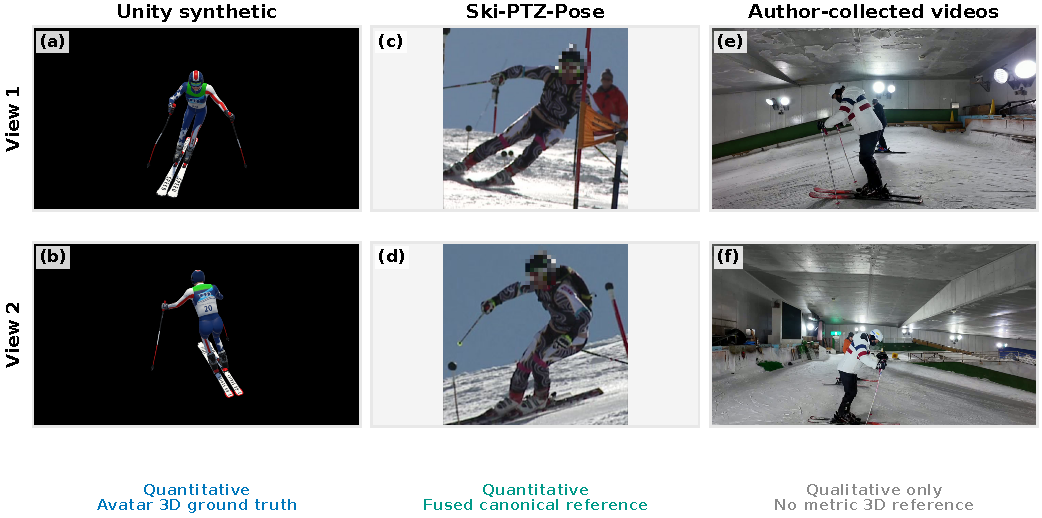
\includegraphics[width=\textwidth]{figures/journal/dataset_examples.pdf}
\caption{Synchronized dual-view examples: (a,b) Unity, (c,d) Ski-PTZ-Pose, (e,f) author-collected videos; rows are the two views. Unity panels are foreground-cropped; the others keep their original field of view.}
\label{fig:dataset_examples}
\end{figure*}

\paragraph{Unity synthetic dataset}
The Unity scene~\cite{juliani2020} contains one female and one male avatar performing steady skiing, braking, falls, and transitions. Table~\ref{tab:dataset_summary} gives the action and camera counts; azimuths are spaced at 10-degree intervals. Each sample comprises one camera pair. Avatar 3D ground truth is independent of the monocular predictions.

\paragraph{Ski-Pose PTZ-Camera dataset}
Ski-PTZ-Pose records competitive giant-slalom skiers with synchronized pan-tilt-zoom cameras and provides 3D poses, projected 2D annotations, and per-frame calibration~\cite{rhodin2018learning,ski_poseptz_dataset}. We align view-specific 3D annotations to a selected camera using similarity transforms fitted on an initial segment. The coordinate-wise median of the aligned annotations on the remaining frames defines the supervision and evaluation reference. Errors measure agreement with this constructed canonical reference, not independent physical 3D accuracy. Neither calibration nor annotation-derived transforms enter CanonFuse3D.

\paragraph{Author-collected qualitative videos}
Six indoor and outdoor dual-view recordings illustrate deployment. Each view is processed independently. These videos have no independent metric 3D annotations and contribute neither training samples nor quantitative evaluation.

\paragraph{Joint convention}
The common 13-joint evaluation set comprises the bilateral shoulders, elbows, hands, hips, knees, and ankles, plus the neck (indices 2--14 of the native 15-joint skeleton). The Unity rig and SAM3D additionally provide two eye landmarks, which help resolve facing direction during canonicalization; Ski-PTZ-Pose and the alternative lifting front ends do not provide these landmarks. The main comparison on both datasets and all cross-front-end comparisons use the common 13 joints. Earlier controlled native-input Unity studies use all 15 joints, whereas the matched RGB-occlusion and calibration study reports common-13 errors after all-15 canonicalization (Section~\ref{subsec:matched_geometry}).

\subsection{Implementation Details}
\label{subsec:implementation_details}

Each camera-pair sample is uniformly resampled to 30 shared frames. The refinement model uses a shared two-layer joint encoder with hidden dimension 128, four-head bidirectional cross-view attention, a depthwise temporal convolution of kernel size 5, and two-layer gate and residual heads, and is trained with AdamW. Unity uses action-disjoint training, validation, and test splits; Ski-PTZ-Pose uses its predefined training and test partitions. Unity model selection uses validation error, while Ski-PTZ-Pose uses predeclared checkpoints because no independent validation partition is available. Test errors do not determine model selection. Complete architectures, optimization settings, split sizes, and checkpoint selection details are provided in Supplementary Section~\ref{S-sec:implementation_record}.

Pose-only controls include the single views, canonical averaging, sequence-aligned averaging~\cite{umeyama1991least}, a 3D quality-weighted average, a temporal convolutional network (TCN) trained on the same data, and SmoothNet~\cite{zeng2022smoothnet} adapted to canonical averaging. The quality heuristic and three-layer, non-dilated TCN are study-specific controls. Temporal convolution has established sequence-modeling precedent~\cite{bai2018empirical}, but our TCN does not reproduce that architecture. SmoothNet's architecture and adaptation settings are documented in the supplement.

Geometric controls comprise classical DLT~\cite{hartley2004multiple}, reprojection-filtered DLT, and DLT with learned residual correction. The latter two are study-specific extensions, not reproductions of published learned-triangulation systems. Their additional estimated 2D observations and calibration are labeled in the main table.

\subsection{Evaluation Metrics}

Errors use the coordinate convention of the corresponding evaluation protocol, without conversion to millimeters. Table~\ref{tab:native_reference} and the controlled canonical-space studies apply the stated body-coordinate transformation independently to predictions and references. Table~\ref{tab:native_output_comparison} instead evaluates admissible native outputs before that transformation and removes only per-frame pelvis translation for position error; PA-MPJPE remains a separate evaluation-only shape alignment. The equations below use the canonical-space notation; the native audit substitutes its declared prediction and reference coordinates. Lower values indicate better agreement with the corresponding reference, and neither coordinate protocols nor dataset reference regimes are pooled.

\subsubsection{Mean per-joint position error}
Mean per-joint position error (MPJPE) averages Euclidean distances between predicted and reference joint positions:
\[
E_{\mathrm{MPJPE}}=\frac{1}{TJ}\sum_{t=1}^{T}\sum_{j=1}^{J}\|P^F_{t,j}-\tilde{G}_{t,j}\|_2.
\]
Dataset-level results aggregate all evaluated joint-frame points. No additional reference alignment is applied for this metric.

\subsubsection{Procrustes-aligned position error}
Procrustes-aligned MPJPE (PA-MPJPE) evaluates pose shape after fitting a least-squares similarity transform from prediction to reference independently in each frame:
\[
E_{\mathrm{PA}}=\frac{1}{TJ}\sum_{t=1}^{T}\sum_{j=1}^{J}\left\|s_t P^F_{t,j}Q_t^{\top}+d_t-\tilde{G}_{t,j}\right\|_2,
\]
where, for each frame \(t\),
\[
(s_t,Q_t,d_t)=\underset{s\geq0,\;Q\in SO(3),\;d\in\mathbb{R}^3}{\arg\min}\;\sum_{j=1}^{J}\left\|sP^F_{t,j}Q^{\top}+d-\tilde{G}_{t,j}\right\|_2^2 .
\]
The fit allows translation, a nonnegative uniform scale, and a proper rotation, with no reflection. Each reported joint subset is aligned separately. Collapsed predictions are mapped to the reference centroid and retained in the average. This reference fit is used only for PA-MPJPE and does not change model inputs, selection, or other metrics.

\subsubsection{Acceleration error}
Acceleration error measures agreement between second-order pose differences:
\[
E_{\mathrm{acc}}=\frac{1}{(T-2)J}\sum_{t=2}^{T-1}\sum_{j=1}^{J}
\|\Delta^2 P^F_{t,j}-\Delta^2\tilde{G}_{t,j}\|_2,
\]
where \(\Delta^2 P_{t,j}=P_{t+1,j}-2P_{t,j}+P_{t-1,j}\). It measures temporal agreement at the evaluated sampling interval, in coordinate units per sampled frame squared.

\subsection{Robustness and Generalization Protocols}
\label{subsec:controlled_protocol}

The robustness studies use the frozen Unity checkpoint and the complete held-out split; additional training is restricted to the explicitly identified gate ablations and front-end adaptation experiments. Camera separation is analyzed in six 30-degree bins of circular azimuth difference between the two cameras. Timing robustness uses seven right-stream offsets from \(-2\) to \(+2\) frames, including half-frame conditions, and seven sampling-rate errors from \(-2\%\) to \(+2\%\); an auxiliary diagnostic additionally estimates larger offsets of up to five frames. Pose-level corruption crosses three affected-view modes, three patterns, and five ratios, giving 45 conditions, and image-level occlusion applies the same view modes and patterns at two ratios to the RGB frames before the native pose estimator, giving 18 conditions; the two ratios parameterize different interventions and do not imply equal physical severity. Front-end generalization replaces SAM3D by three lifting estimators applied to the same ground-truth 2D tracks, isolating the lifting stage, followed by frozen transfer and target-specific or mixed adaptation. Finally, the multi-view extension composes the frozen dual-view model over all camera pairs of nested one- to four-camera groups. Full intervention and aggregation rules are given in Supplementary Section~\ref{S-sec:controlled_details}.

A separate matched-input study compares five frozen methods on clean images and random ratio-0.5/1.0 masks applied to the left, right, or both views. Paired estimated 2D and 3D observations come from the same SAM3D detections. The geometry-assisted methods additionally receive calibration, with right-camera extrinsic rotation perturbations of $0^\circ$, $1^\circ$, and $3^\circ$. All seven conditions retain the full test cohort, including detection failures (Section~\ref{subsec:matched_geometry}).

\section{Results}
\label{sec:results}

\subsection{Primary performance and cross-dataset evidence}

Table~\ref{tab:native_reference} compares CanonFuse3D with the pose-only fusion baselines, adapted published methods, and the separately labeled geometric group on the common 13-joint subset of both datasets after the shared body-coordinate normalization. On all 64,440 held-out Unity camera-pair sequences, CanonFuse3D reduces MPJPE from 0.2792 for canonical averaging to 0.1551 (44.5\%). Within this canonical-space protocol, the right row has larger MPJPE than the left row (0.4617 versus 0.1624). This gap cannot by itself be attributed to worse native front-end predictions because the streams pass through separate batch-referenced coordinate transforms; the native-output audit below evaluates the upstream predictions in declared frames. Aligning the right stream to the left before averaging reduces the canonical-space error to 0.1622, and the quality-weighted average brings no further gain. CanonFuse3D improves on the best of these non-learned methods in MPJPE (0.1551 versus 0.1622), PA-MPJPE (0.0637 versus 0.0667), and acceleration error (0.0297 versus 0.0308), so the learned fusion adds accuracy and temporal stability beyond what pose-space alignment alone provides. It is also more accurate than the temporal convolutional baseline trained on the same data (0.1610 MPJPE, 0.0690 PA-MPJPE, 0.0339 acceleration error). SmoothNet applied to canonical averaging gives the lowest acceleration error in the group (0.0113) but leaves the position error at 0.2925, so temporal smoothness and positional accuracy must be read separately. On all 15 Unity joints, the corresponding reduction over canonical averaging is 46.3\% (0.1541 versus 0.2868; Supplementary Table~\ref{S-tab:native_reference_all15}).

On the 30 fixed Ski-PTZ-Pose test sequences, the two views disagree far more (0.3552 and 0.4462), and pose-space alignment alone does not resolve the disagreement (0.3537). CanonFuse3D reduces MPJPE to 0.1794, a 48.6\% reduction over canonical averaging, with PA-MPJPE 0.1269 and acceleration error 0.0311. On this small real-world index the temporal convolutional baseline reaches lower MPJPE and PA-MPJPE (0.1581 and 0.1144) at a higher acceleration error (0.0411), and SmoothNet again gives the lowest acceleration error (0.0151) with a position error close to averaging (0.3227). These values measure agreement with the constructed annotation reference.

The geometric group quantifies what calibration buys. With the estimated 2D joints and the supplied calibration, plain DLT is less accurate than CanonFuse3D on both datasets (0.1983 and 0.3984), reprojection gating does not improve it, and only a learned residual correction on top of DLT reaches lower MPJPE (0.0964 and 0.1643), at the cost of 2D observations and camera calibration that the pose-only setting excludes; this group is therefore not a common-input comparison. On Ski-PTZ-Pose the geometric predictions are first centered at their own per-frame pelvis, consistent with the root-relative annotations, without fitting anything to the test reference.

The published adaptations give a metric-dependent comparison under their stated contracts. Avg.~+~STRIDE~\cite{lal2025stride} remains close to canonical averaging, with Unity MPJPE 0.2799, PA-MPJPE 0.1174, and acceleration error 0.0316; its corresponding Ski-PTZ-Pose values are 0.3483, 0.1861, and 0.0387. The official-protocol DeciWatch adaptation~\cite{zeng2022deciwatch} reaches 0.1134, 0.0695, and 0.0132 on Unity and 0.2239, 0.1549, and 0.0168 on Ski-PTZ-Pose. It has lower Unity MPJPE and acceleration error than CanonFuse3D but higher PA-MPJPE; on Ski-PTZ-Pose, CanonFuse3D has lower MPJPE and PA-MPJPE while DeciWatch has lower acceleration error. MetaPose~\cite{usman2022metapose}, which additionally uses estimated 2D joints, reaches 0.2655, 0.1089, and 0.0400 on Unity and 0.4253, 0.1425, and 0.0634 on Ski-PTZ-Pose. These adapted methods differ in input, supervision, and temporal-recovery task, so the table reports their outcomes without treating the lowest cell in each column as a common-input winner.

\begin{table*}[t]
\centering
\caption{Comparison after the shared body-coordinate normalization on the common 13 joints (Unity: all 64,440 held-out camera pairs; Ski-PTZ-Pose: all 30 fixed test sequences). Published adaptations are separated because their input and task budgets differ: STRIDE refines the canonical average, DeciWatch recovers 30 frames from four, and MetaPose also receives estimated 2D joints. Bold marks the lowest value within each input block.}
\label{tab:native_reference}
\small
\setlength{\tabcolsep}{4pt}
\resizebox{\linewidth}{!}{%
\begin{tabular}{@{}lrrrrrr@{}}
\toprule
& \multicolumn{3}{c}{Unity} & \multicolumn{3}{c}{Ski-PTZ-Pose} \\
\cmidrule(lr){2-4}\cmidrule(lr){5-7}
Method & MPJPE $\downarrow$ & PA-MPJPE $\downarrow$ & Accel. $\downarrow$ & MPJPE $\downarrow$ & PA-MPJPE $\downarrow$ & Accel. $\downarrow$ \\
\midrule
\multicolumn{7}{@{}l}{\textit{3D pose inputs only}} \\
Left canonical & 0.1624 & 0.0711 & 0.0355 & 0.3552 & 0.1864 & 0.0531 \\
Right canonical & 0.4617 & 0.0759 & 0.0452 & 0.4462 & 0.1754 & 0.0455 \\
Canonical average & 0.2792 & 0.1162 & 0.0322 & 0.3487 & 0.1877 & 0.0392 \\
Aligned average~\cite{umeyama1991least} & 0.1622 & 0.0667 & 0.0308 & 0.3537 & 0.1718 & 0.0381 \\
3D quality-weighted fusion & 0.2767 & 0.1152 & 0.0312 & 0.3499 & 0.1875 & 0.0385 \\
% Cross-view MLP & 0.1361 & 0.0561 & 0.0312 & 0.1423 & 0.1045 & 0.0315 \\
Temporal fusion (local TCN)~\cite{bai2018empirical} & 0.1610 & 0.0690 & 0.0339 & \textbf{0.1581} & \textbf{0.1144} & 0.0411 \\
Avg. + SmoothNet~\cite{zeng2022smoothnet} & 0.2925 & 0.1860 & \textbf{0.0113} & 0.3227 & 0.1924 & \textbf{0.0151} \\
\addlinespace[2pt]
\multicolumn{7}{@{}l}{\textit{Published temporal adaptations of the canonical average}} \\
Avg. + STRIDE (adapted)~\cite{lal2025stride} & 0.2799 & 0.1174 & 0.0316 & 0.3483 & 0.1861 & 0.0387 \\
DeciWatch (official-protocol adaptation)~\cite{zeng2022deciwatch} & 0.1134 & 0.0695 & 0.0132 & 0.2239 & 0.1549 & 0.0168 \\
\addlinespace[2pt]
\multicolumn{7}{@{}l}{\textit{Proposed pose-only fusion}} \\
CanonFuse3D (ours) & \textbf{0.1551} & \textbf{0.0637} & 0.0297 & 0.1794 & 0.1269 & 0.0311 \\
\midrule
\multicolumn{7}{@{}l}{\textit{Additional estimated 2D joints without camera calibration}} \\
MetaPose (adapted)~\cite{usman2022metapose} & 0.2655 & 0.1089 & 0.0400 & 0.4253 & 0.1425 & 0.0634 \\
\addlinespace[2pt]
\multicolumn{7}{@{}l}{\textit{Additional estimated 2D joints and camera calibration}} \\
Calibrated DLT~\cite{hartley2004multiple} & 0.1983 & 0.1146 & 0.0376 & 0.3984 & 0.2219 & 0.0816 \\
Reprojection-gated DLT~\cite{hartley2004multiple} & 0.2088 & 0.1196 & \textbf{0.0295} & 0.3996 & 0.2234 & 0.0846 \\
DLT-residual MLP~\cite{hartley2004multiple} & \textbf{0.0964} & \textbf{0.0535} & 0.0403 & \textbf{0.1643} & \textbf{0.1172} & \textbf{0.0598} \\
\bottomrule
\end{tabular}}
\end{table*}

\begin{table*}[t]
\centering
\caption{Unity comparison before the shared body-coordinate normalization, with every method in its native output frame. Position error removes only per-frame pelvis translation; Procrustes alignment is a separate reflection-free diagnostic. A double dash marks the absence of a target-independent common frame.}
\label{tab:native_output_comparison}
\footnotesize
\setlength{\tabcolsep}{4pt}
\begin{tabular}{@{}lrrr@{}}
\toprule
Method & MPJPE $\downarrow$ & PA-MPJPE $\downarrow$ & Accel. $\downarrow$ \\
\midrule
\multicolumn{4}{@{}l}{\textit{Native monocular front ends}} \\
SAM 3D Body~\cite{yang2026sam} & 0.1019 & 0.0732 & 0.0369 \\
MotionBERT~\cite{zhu2023motionbert} & 0.2553 & 0.1150 & 0.0090 \\
PoseFormer~\cite{zheng2021poseformer} & 0.2075 & 0.1371 & 0.0068 \\
VideoPose3D~\cite{pavllo2019videopose3d} & 0.1583 & 0.1028 & 0.0076 \\
\addlinespace[2pt]
\multicolumn{4}{@{}l}{\textit{Pre-Canon controls}} \\
Left native & 0.0967 & 0.0708 & 0.0333 \\
Right native & 0.1070 & 0.0756 & 0.0406 \\
Unaligned native average & -- & -- & -- \\
Sequence-aligned average~\cite{umeyama1991least} & 0.0970 & 0.0666 & 0.0285 \\
Aligned quality-weighted fusion & 0.0960 & 0.0660 & 0.0276 \\
Aligned average + SmoothNet~\cite{zeng2022smoothnet} & -- & -- & -- \\
\addlinespace[2pt]
\multicolumn{4}{@{}l}{\textit{Published external methods}} \\
STRIDE (per-view adaptation)~\cite{lal2025stride} & 0.1072 & 0.0776 & 0.0357 \\
DeciWatch (per-view adaptation)~\cite{zeng2022deciwatch} & 0.6315 & 0.3033 & 0.0119 \\
MetaPose (adapted)~\cite{usman2022metapose} & 0.2171 & 0.1088 & 0.0382 \\
\addlinespace[2pt]
\multicolumn{4}{@{}l}{\textit{Calibrated geometry}} \\
Calibrated DLT~\cite{hartley2004multiple} & 0.1705 & 0.1072 & 0.0614 \\
Reprojection-gated DLT~\cite{hartley2004multiple} & 0.1711 & 0.1098 & 0.0520 \\
DLT-residual MLP~\cite{hartley2004multiple} & -- & -- & -- \\
\bottomrule
\end{tabular}
\end{table*}


Table~\ref{tab:native_output_comparison} instead evaluates outputs before the shared body-coordinate normalization. On Unity, the pooled native SAM3D streams have MPJPE/PA-MPJPE/acceleration error 0.1019/0.0732/0.0369. The native left stream is slightly more accurate than the right (0.0967 versus 0.1070 MPJPE), while sequence alignment and quality weighting reduce PA-MPJPE to 0.0666 and 0.0660. Among the published-method adaptations, per-view STRIDE~\cite{lal2025stride} reaches 0.1072/0.0776/0.0357, per-view DeciWatch~\cite{zeng2022deciwatch} reaches 0.6315/0.3033/0.0119, and MetaPose~\cite{usman2022metapose} reaches 0.2171/0.1088/0.0382. DeciWatch therefore smooths its per-view inputs but incurs large position error under this native-view application; this row is distinct from the canonical-average recovery protocol in Table~\ref{tab:native_reference}.

Table~\ref{tab:native_output_comparison} scores every method in its declared output frame without the body-coordinate transform: monocular and temporal-refinement rows pool independently scored left and right streams, MetaPose stays in its restored left-camera frame, and calibrated geometry stays in its supplied world frame. Ski-PTZ-Pose is omitted because its constructed reference has no independently supplied mapping into these frames, and CanonFuse3D appears only in the canonical-space table. Because the two tables differ in whether the shared normalization is applied, methods must not be ranked across the two tables.

\FloatBarrier
\subsection{Reliability-gate behavior}

Table~\ref{tab:gate_retraining} crosses dynamic versus fixed-0.5 gating with presence versus absence of the output residual. The three learned configurations are retrained from scratch under the benchmark protocol (Supplementary Section~\ref{S-sec:gate_audit}); the fourth has no trainable output path. This full-model control is distinct from the archived benchmark checkpoint, on which the subsequent interventions act.

\begin{table}[htbp]
\centering
\caption{Gate and output-residual ablation on Unity (common 13, canonical coordinates). Each learned configuration is trained from scratch with the same seed, split, budget, and selection rule; lower is better.}
\label{tab:gate_retraining}
\small
\setlength{\tabcolsep}{5pt}
\begin{tabular}{llrrr}
\toprule
Gate & Output residual & MPJPE & PA-MPJPE & Accel. \\
\midrule
Dynamic & Learned & \textbf{0.14639} & \textbf{0.06734} & 0.02953 \\
Fixed 0.5 & Learned & 0.17279 & 0.07011 & 0.03012 \\
Dynamic & None & 0.16334 & 0.07337 & 0.02929 \\
Fixed 0.5 & None (deterministic) & 0.27997 & 0.11486 & \textbf{0.02513} \\
\bottomrule
\end{tabular}
\end{table}


With the output residual retained, learned gating lowers MPJPE from 0.17279 to 0.14639 (15.3\%) relative to fixed weights; with dynamic gating retained, the output residual lowers MPJPE from 0.16334 to 0.14639 (10.4\%). The full model also has the lowest PA-MPJPE, so gating and residual correction contribute complementary position accuracy under this protocol. Removing the residual slightly lowers acceleration error, and the deterministic configuration is smoothest but has the largest position error.

In the frozen benchmark model, each gated candidate already combines both aligned raw views, so \(\alpha=1\) or 0 does not select an isolated camera. On all 15 Unity joints, the correlation between \(\alpha\) and right-minus-left candidate error is 0.651, and the larger weight selects the lower-error candidate in 91.7\% of non-tied joint-frame comparisons (Table~\ref{tab:gate_region_summary}, Fig.~\ref{fig:gate_diagnostics_full}). The mean left-candidate weight is 0.6804, with small across-joint variation but a joint-frame standard deviation of 0.1122. These are diagnostics of aligned-candidate errors in evaluation coordinates, not probabilistic calibration.

\begin{table}[t]
\centering
\caption{Region-wise reliability-gate statistics on the complete Unity test split without masking.}
\label{tab:gate_region_summary}
\footnotesize
\setlength{\tabcolsep}{6pt}
\renewcommand{\arraystretch}{1.08}
\begin{tabular}{lccc}
\toprule
Region & Joints & \(\alpha\) & \(1-\alpha\) \\
\midrule
Upper limbs & 6 & \(0.6879 \pm 0.0132\) & 0.3121 \\
Lower limbs & 6 & \(0.6686 \pm 0.0103\) & 0.3314 \\
All joints & 15 & \(0.6804 \pm 0.0144\) & 0.3196 \\
\bottomrule
\end{tabular}
\vspace{0.4em}
\begin{minipage}{0.94\linewidth}
\footnotesize
\textit{Note.} Mean and across-joint standard deviation of per-joint mean \(\alpha\). Upper limbs are the six shoulder, elbow, and wrist joints; lower limbs the six hip, knee, and ankle joints; all joints additionally include both eyes and the neck.
\end{minipage}
\end{table}

\FloatBarrier
\begin{figure}[htbp]
\centering
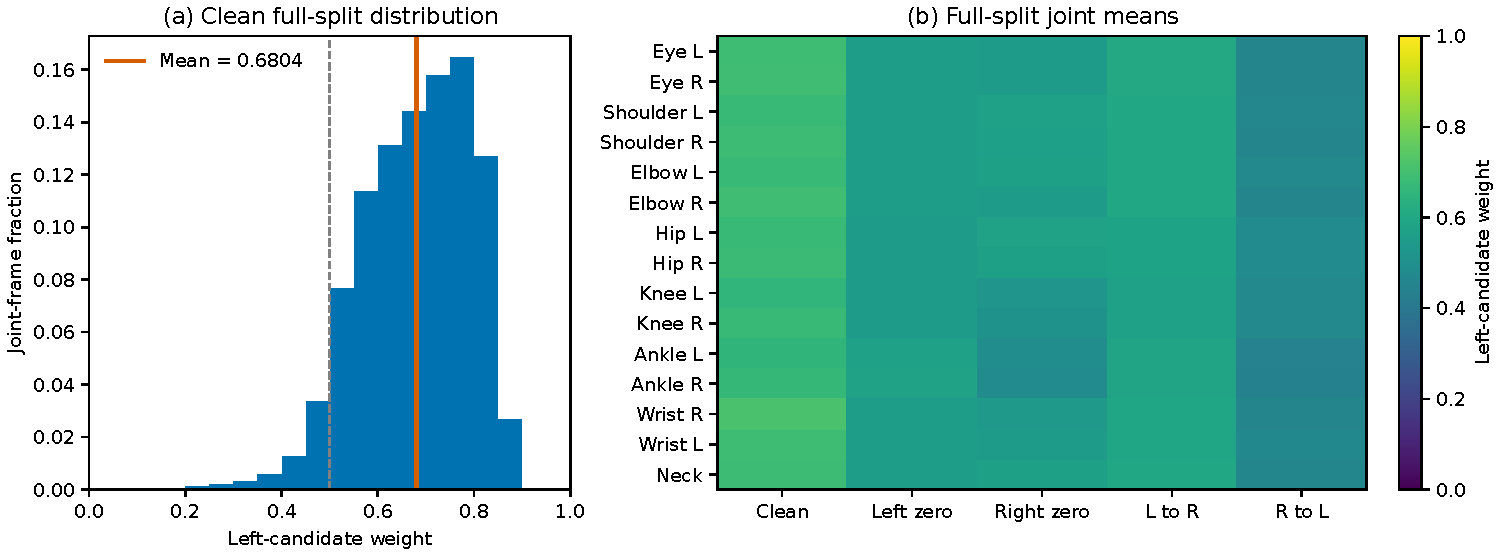
\includegraphics[width=\linewidth]{figures/journal/gate_diagnostics_full.pdf}
\caption{Frozen-checkpoint gate diagnostics on the complete Unity split (all 15 joints): (a) clean joint-frame weight distribution; (b) per-joint means under clean inputs, complete zeroing of either stream, and midpoint switches of the zeroed stream.}
\label{fig:gate_diagnostics_full}
\end{figure}

Freezing this checkpoint and replacing only the gate by 0.5 raises clean common-13 MPJPE from 0.1551 to 0.2104 on Unity and from 0.1794 to 0.1842 on Ski-PTZ-Pose. Under complete raw-pose zeroing and midpoint switches, the original checkpoint retains only a small advantage over the fixed-gate intervention, and on Unity it is worse than canonical averaging in every such condition. Turning off its output residual reduces Unity error under these extreme perturbations but worsens clean error and all tested Ski conditions. Because complete zeroing also disrupts the batch anchor and Sim3 alignment, these results do not establish automatic recovery of a missing view. All interventions are reported in Supplementary Table~\ref{S-tab:gate_frozen_interventions} and Fig.~\ref{S-fig:gate_fixed_examples}.

\FloatBarrier
\subsection{Camera-pair separation}

The controlled studies in this and the following three subsections vary one capture condition at a time with the checkpoint, split, and evaluation path fixed. The camera-angle breakdown in Table~\ref{tab:view_angle} reveals no failure regime: CanonFuse3D MPJPE decreases from 0.1563 in the 0--30 degree bin to 0.1528 around 120--150 degrees, while the gain over canonical averaging stays between 45.9\% and 46.6\%. Wider separation therefore supplies slightly more complementary evidence, but the narrow range does not support a strong optimum.

\begin{table}[t]
\centering
\caption{Accuracy and camera-pair bootstrap intervals by azimuth separation. Positive gain favors CanonFuse3D.}
\label{tab:view_angle}
\small
\setlength{\tabcolsep}{4pt}
\resizebox{\linewidth}{!}{%
\begin{tabular}{lrrrrl}
\toprule
Angle (deg) & Pairs & Canon. avg. & Fused & Mean gain & 95\% CI \\
\midrule
0--30 & 2,160 & 0.2891 & 0.1563 & 0.1328 & [0.1313, 0.1343] \\
30--60 & 2,700 & 0.2888 & 0.1554 & 0.1334 & [0.1321, 0.1347] \\
60--90 & 2,700 & 0.2876 & 0.1544 & 0.1332 & [0.1318, 0.1345] \\
90--120 & 2,700 & 0.2865 & 0.1529 & 0.1337 & [0.1324, 0.1349] \\
120--150 & 2,700 & 0.2852 & 0.1528 & 0.1325 & [0.1314, 0.1336] \\
150--180 & 3,150 & 0.2844 & 0.1532 & 0.1312 & [0.1303, 0.1322] \\
\bottomrule
\end{tabular}}
\vspace{0.3em}
\begin{minipage}{0.97\linewidth}
\footnotesize\textit{Note.} Each camera pair contributes four action-specific sequences; the bins cover all 64,440 test sequences. MPJPE and absolute gain use dataset coordinate units. Intervals resample camera pairs. Detailed paired tests and effect sizes appear in Supplementary Table~\ref{S-tab:view_angle_significance}.
\end{minipage}
\end{table}


Collapsing the four action-specific observations of each camera geometry into one unordered pair, every angle bin retains a positive fusion gain under paired Wilcoxon testing (Holm-adjusted \(p<0.001\); rank-biserial correlation 0.994--1.000). The across-bin Kruskal--Wallis test is significant (\(p=0.025\)) with a negligible effect size (\(\epsilon^2=0.00049\)), and only one of 15 Holm-adjusted post-hoc comparisons, 90--120 versus 150--180 degrees, remains significant (\(p=0.0064\), \(r_{rb}=0.053\)). The fusion benefit is thus reliable within every bin, whereas camera separation explains little of its magnitude (Supplementary Table~\ref{S-tab:view_angle_significance}, Fig.~\ref{S-fig:view_angle_extension}).

\FloatBarrier
\subsection{Temporal offset and sampling-rate drift}

Figure~\ref{fig:temporal_sampling} summarizes two synchronization stress tests as relative MPJPE changes from each method's unperturbed value; Supplementary Table~\ref{S-tab:temporal_sampling} gives absolute errors and gate diagnostics. Across \(\pm2\) frame offsets, all-15 MPJPE ranges from 0.1537 to 0.1555 around the unperturbed 0.1541; the worst case, a two-frame positive offset, is 0.91\% above zero. Gate-error correlation stays between 0.646 and 0.650 and view-preference accuracy above 91.4\%, so sequence-level alignment and the five-frame temporal refiner tolerate short local disagreement.

Clock-rate perturbations are smaller still: MPJPE rises by 0.23\% at \(+2\%\) and changes by less than 0.02\% for negative perturbations up to \(-2\%\). Acceleration error is not monotonic because resampling smooths as well as misaligns trajectories, so MPJPE is the cleaner measure of rate-drift sensitivity.

\begin{figure}[!htb]
\centering
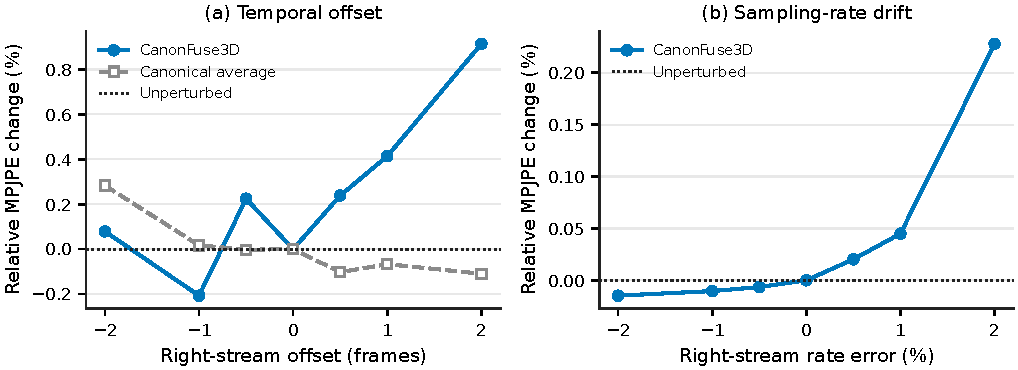
\includegraphics[width=0.9\linewidth]{figures/extension/temporal_sampling.pdf}
\caption{Relative MPJPE change under right-stream temporal offset and sampling-rate error, each curve normalized by its own unperturbed MPJPE; dotted lines mark zero change.}
\label{fig:temporal_sampling}
\end{figure}

\FloatBarrier
\subsection{Missing-pose evidence}

Figure~\ref{fig:masking_extension} reports all 45 conditions of the missing-pose study under the corruption protocol of Supplementary Section~\ref{S-sec:controlled_details}; Supplementary Table~\ref{S-tab:masking_extension} lists exact errors and gains at ratios 0.5 and 1.0.

Single-view corruption tests whether the complementary stream can rescue degraded evidence, whereas both-view corruption removes that redundancy. At ratio 0.5, single-view temporal masking retains gains of 37.0\% (left) and 37.9\% (right) over canonical averaging, and distal masking 28.0\% and 31.5\%; the advantage narrows for unstructured random corruption. When random corruption affects both streams at ratio 0.5, fusion is 3.3\% worse than canonical averaging, whereas bilateral temporal and distal corruption still retain gains of 26.9\% and 12.5\%. The checkpoint therefore exploits a clean complementary stream and structured missingness, but dense independent corruption of both inputs lies outside its reliable regime.

\begin{figure}[!htb]
\centering
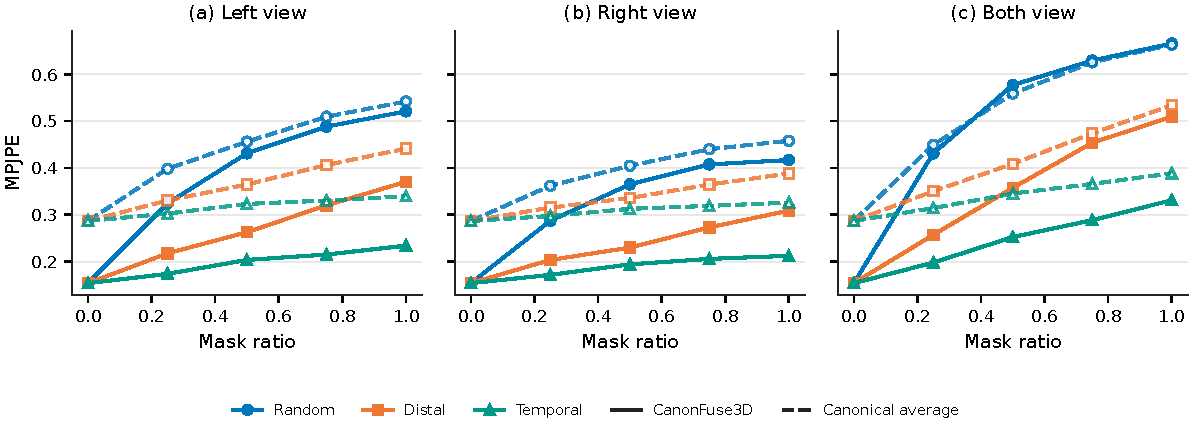
\includegraphics[width=0.98\linewidth]{figures/extension/masking_robustness.pdf}
\caption{Complete held-out-split masking robustness for left-, right-, and both-view corruption.}
\label{fig:masking_extension}
\end{figure}

\FloatBarrier
\subsection{Image-level occlusion through the pose front end}

Figure~\ref{fig:image_occlusion_examples} illustrates the three image-level occlusion patterns, which place mean-color patches on the projected joints selected by the same random, distal, and temporal rules as the pose-level study before SAM3D inference (Supplementary Section~\ref{S-sec:controlled_details}). The resulting errors therefore include missed detections and distorted poses produced by the front end; Supplementary Table~\ref{S-tab:image_occlusion} lists all 18 conditions.

\begin{figure}[!htb]
\centering
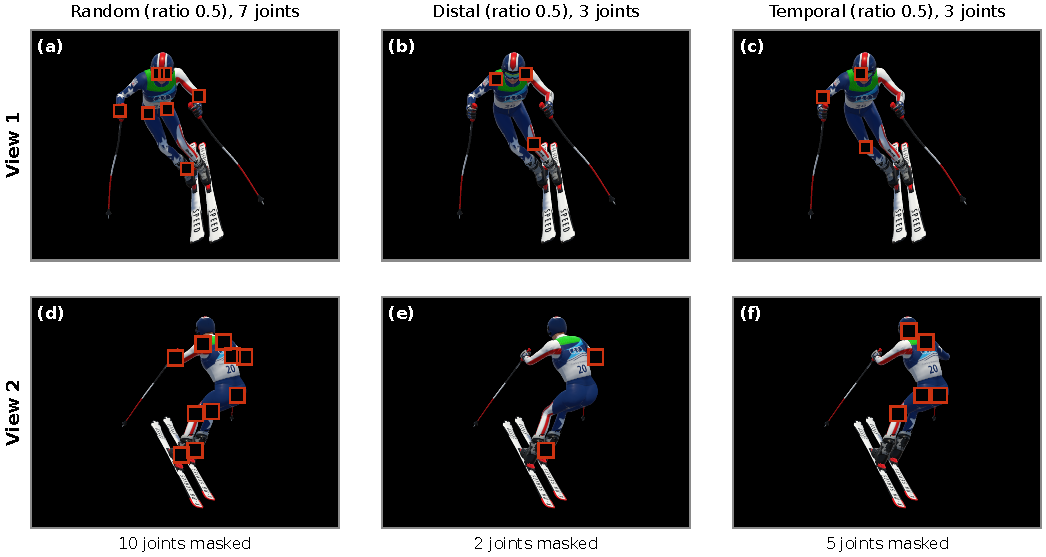
\includegraphics[width=0.98\linewidth]{figures/journal/image_occlusion_examples.pdf}
\caption{Image-level occlusion on one Unity frame: rows are the two views, columns the random, distal, and temporal patterns at ratio 0.5. Red outlines mark the mean-color patches (drawn for illustration only); panel labels give the number of masked joints.}
\label{fig:image_occlusion_examples}
\end{figure}

CanonFuse3D improves on canonical averaging in 15 of the 18 conditions. At random ratio 0.5, gains are 31.9\%, 34.3\%, and 20.9\% for left-, right-, and both-view occlusion, and all twelve distal and temporal conditions retain gains of 14.6--43.4\% and 42.3--45.9\%, respectively. The robustness evidence thus extends to errors produced by the image-to-pose front end.

Random occlusion at ratio 1.0 reverses the advantage in all three view modes: fused MPJPE exceeds canonical averaging by 18.0\%, 9.2\%, and 28.4\% for left, right, and both views. In the bilateral case, MPJPE is 0.6311 versus 0.4914 with a pair-aligned SAM3D detection-failure rate of 36.36\% (40.51\% and 32.22\% for the left- and right-view conditions). Failed detections remain in the evaluation as zero poses, so an unoccluded complementary view does not guarantee a fusion advantage under this severe intervention.

Figure~\ref{fig:image_occlusion_extension} compares fused MPJPE under image-level and direct pose-stream interventions. Matching ratios control different perturbations: bilateral random corruption at ratio 0.5 retains a 20.9\% gain in the image-level experiment but gives a 3.3\% disadvantage in the pose-level experiment. The two protocols therefore probe distinct error distributions and do not define an ordering of physical occlusion severity.

\begin{figure}[!htb]
\centering
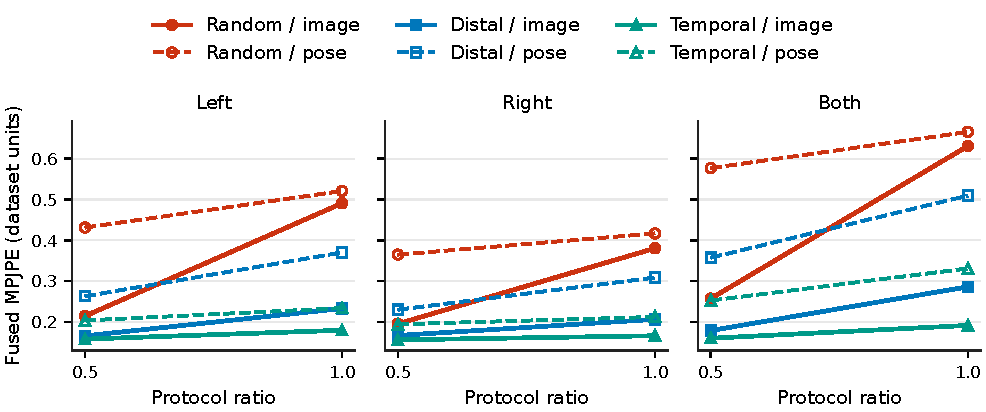
\includegraphics[width=0.98\linewidth]{figures/extension/image_occlusion_robustness.pdf}
\caption{Fused MPJPE under image-level occlusion (solid, filled markers) and direct pose-stream corruption (dashed, open markers) for left-, right-, and both-view interventions. Matching ratios do not imply equal physical severity.}
\label{fig:image_occlusion_extension}
\end{figure}

\FloatBarrier
\subsection{Matched occlusion and calibration sensitivity}
\label{subsec:matched_geometry}

We compare pose-only fusion with geometry-assisted reconstruction on predictions from the same corrupted images, following the matched protocol of Section~\ref{subsec:controlled_protocol} and Supplementary Section~\ref{S-sec:c07_matched_geometry}: one SAM3D call supplies both the projected 2D keypoints and the 3D pose of the same person, all five frozen methods retain the same 64,440 windows, and scoring uses the common 13 joints after all-15 canonicalization. This seven-condition study uses fresh paired predictions and a different joint subset from the preceding 18-condition study, so their numbers are not interchangeable.

\begin{table}[htbp]
\centering
\caption{Matched RGB-occlusion comparison on Unity, with supplied calibration and no added extrinsic perturbation. Common-13 canonical MPJPE (lower is better), on all 64,440 windows. Ratios select joints for patch placement, not image-area coverage.}
\label{tab:c07_occlusion_mpjpe}
\small
\setlength{\tabcolsep}{4pt}
\begin{tabular}{lrrrrr}
\toprule
Condition & CanonFuse3D & Average & DLT & Gated DLT & DLT-residual \\
\midrule
Clean & 0.1553 & 0.2797 & 0.2004 & 0.2108 & 0.0988 \\
Left 0.5 & 0.2103 & 0.3051 & 0.2542 & 0.2606 & 0.1498 \\
Right 0.5 & 0.1949 & 0.2890 & 0.2488 & 0.2556 & 0.1417 \\
Both 0.5 & 0.2514 & 0.3146 & 0.2957 & 0.2983 & 0.1870 \\
Left 1.0 & 0.4654 & 0.3992 & 0.4499 & 0.4495 & 0.3569 \\
Right 1.0 & 0.3706 & 0.3347 & 0.5501 & 0.4569 & 0.4070 \\
Both 1.0 & 0.5986 & 0.4654 & 0.5121 & 0.4866 & 0.4155 \\
\bottomrule
\end{tabular}
\par\smallskip\begin{minipage}{\linewidth}\footnotesize CanonFuse3D and canonical averaging use only predicted 3D. The three DLT-based methods additionally use estimated 2D and calibration. DLT follows~\cite{hartley2004multiple}; gating and the residual MLP are study-specific controls, not reproductions of published learned triangulation systems.\end{minipage}
\end{table}



With unperturbed supplied calibration (Table~\ref{tab:c07_occlusion_mpjpe}), DLT-residual has the lowest MPJPE in six of seven conditions: its clean error is 0.0988 versus 0.1553 for CanonFuse3D, and under the three ratio-0.5 masks its MPJPE is 25.6--28.8\% lower, whereas CanonFuse3D has 1.8--9.5\% lower PA-MPJPE and 43.7--46.0\% lower acceleration error. The additional-input method thus improves position accuracy, while the pose-only method retains advantages on aligned configuration and temporal second-difference error. CanonFuse3D also improves MPJPE over canonical averaging by 20.1--32.5\% under ratio-0.5 masks, but at ratio 1.0 this advantage reverses by 10.7--28.6\% for single-side and bilateral masking alike; the results do not support automatic rejection of an arbitrarily degraded input view.

\begin{figure}[htbp]
\centering
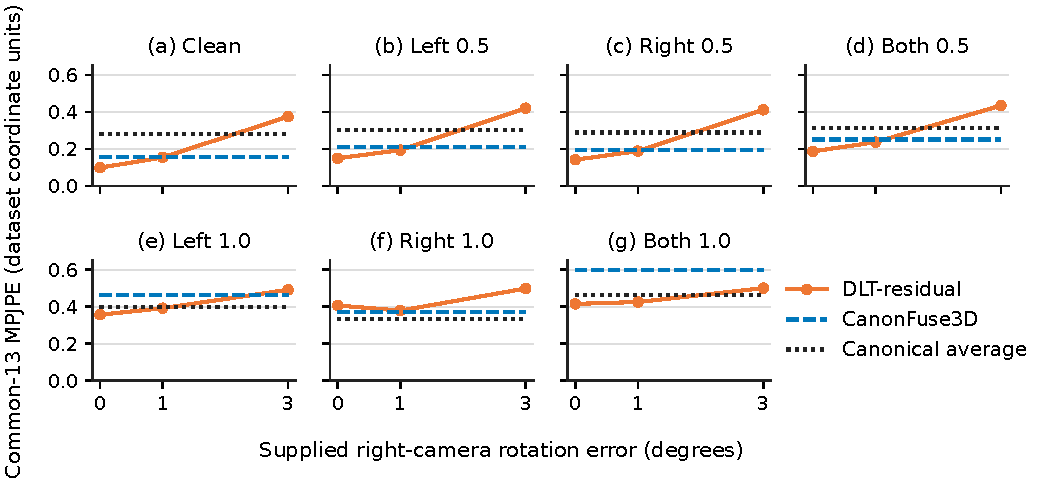
\includegraphics[width=\linewidth]{figures/extension/c07_calibration_sensitivity.pdf}
\caption{Calibration sensitivity across the seven matched conditions. Markers show DLT-residual~\cite{hartley2004multiple} at the three tested angles; pose-only references are unchanged. The synthetic rotation affects only the supplied right-camera orientation (values in Supplementary Table~\ref{S-tab:c07_calibration_mpjpe}).}
\label{fig:c07_calibration}
\end{figure}

Figure~\ref{fig:c07_calibration} shows the effect of perturbing the supplied right-camera extrinsics by $0^\circ$, $1^\circ$, and $3^\circ$ with the left camera and the right-camera center fixed. DLT-residual still has lower MPJPE than CanonFuse3D on clean and ratio-0.5 inputs at $1^\circ$. At $3^\circ$, CanonFuse3D has the lowest MPJPE and PA-MPJPE among the five methods on those four conditions, whereas canonical averaging is best on both metrics in all three ratio-1.0 conditions. Pose-only scores are invariant because neither their images nor their 3D inputs change; the experiment measures sensitivity to supplied calibration, not to physically moving a camera.

Missing observations remain in all denominators. At bilateral ratio 1.0, at least one view fails in 54.85\% of pair--frame positions, and after the batch-referenced transformation 33.30\% of CanonFuse3D and 70.05\% of DLT and gated-DLT frames have collapsed common-13 configurations, since a missing reference frame can affect an entire batch. These results characterize the coupled front-end, fallback, normalization, and prediction pipeline.

\FloatBarrier


\subsection{Front-end generalization and adaptation}

CanonFuse3D is trained on SAM3D streams, but the framework is front-end agnostic: it consumes only 3D pose sequences on the common joint set. Table~\ref{tab:frontend_generalization} evaluates the frozen SAM3D-trained checkpoint on three alternative lifting front ends without retraining. MotionBERT retains a positive gain of 8.0\% over its own canonical average, whereas PoseFormer and VideoPose3D degrade by 18.0\% and 12.8\%. Canonicalization removes global position and orientation differences but not estimator-specific limb bias and temporal statistics, so a frozen model remains coupled to the error distribution it was trained on and transfer to a new estimator must be validated.

\begin{table}[t]
\centering
\caption{Frozen transfer to alternative upstream estimators on the common 13-joint subset. Lower MPJPE is better. Gain is relative to canonical averaging; positive values indicate improvement.}
\label{tab:frontend_generalization}
\small
\setlength{\tabcolsep}{4pt}
\begin{tabular}{lrrrr}
\toprule
Front end & Canon. avg. & Fused & Gain (\%) & Gate pref. (\%) \\
\midrule
MotionBERT & 0.4766 & 0.4385 & +8.0 & 61.4 \\
PoseFormer & 0.4542 & 0.5360 & -18.0 & 52.3 \\
VideoPose3D & 0.4776 & 0.5389 & -12.8 & 47.0 \\
\bottomrule
\end{tabular}
\end{table}


\IfFileExists{tables/frontend_adaptation.tex}{%
Lightweight adaptation restores the benefit on every front end. Table~\ref{tab:frontend_adaptation} reports the complete \(8\times4\) matrix in which the frozen reference checkpoint and seven adapted models are evaluated on all four front ends (relative recovery in Supplementary Fig.~\ref{S-fig:frontend_adaptation}). Each adaptation updates either the gate and residual heads or all parameters for 20 epochs on training and validation actions only. Full target-specific adaptation reduces the matched-front-end error to 0.2290 for VideoPose3D, 0.2741 for PoseFormer, and 0.2393 for MotionBERT, which is 52.0\%, 39.7\%, and 49.8\% below the canonical average of the respective front end (0.4776, 0.4542, and 0.4766) and 57.5\%, 48.9\%, and 45.4\% below the frozen checkpoint on the same input. A single model adapted on a balanced mixture of all four front ends reaches 0.2363, 0.2751, and 0.2464 on the three alternatives while retaining 0.1809 on SAM3D, 16.7\% above the native checkpoint but 35.2\% below canonical averaging. One architecture, adapted with a short schedule, therefore improves over canonical averaging on every tested front end; the remaining trade-off is between recovery on the target front end and retention on the native one.
\begin{table*}[t]
\centering
\caption{Common-13 MPJPE after front-end-specific or mixed adaptation. Each row is one frozen model evaluated on all four front ends; lower is better.}
\label{tab:frontend_adaptation}
\small
\begin{tabular}{lrrrr}
\toprule
Adaptation model & SAM3D & VideoPose3D & PoseFormer & MotionBERT \\
\midrule
Frozen reference & 0.1551 & 0.5389 & 0.5360 & 0.4385 \\
\midrule
VideoPose3D/heads & 0.2120 & 0.2621 & 0.3297 & 0.3567 \\
VideoPose3D/full & 0.2442 & 0.2290 & 0.2954 & 0.4403 \\
PoseFormer/heads & 0.1822 & 0.2833 & 0.3234 & 0.3521 \\
PoseFormer/full & 0.2033 & 0.2447 & 0.2741 & 0.3381 \\
MotionBERT/heads & 0.1976 & 0.4667 & 0.5100 & 0.2744 \\
MotionBERT/full & 0.2117 & 0.5050 & 0.6036 & 0.2393 \\
Mixed/full & 0.1809 & 0.2363 & 0.2751 & 0.2464 \\
\bottomrule
\end{tabular}
\end{table*}


}{%
\paragraph{Pending result} Front-end adaptation results will be inserted only after all seven training runs and all 32 test cells pass the no-leakage and full-split validators.
}

\FloatBarrier
\subsection{Scaling beyond two views}

\IfFileExists{tables/nview_scaling.tex}{%
Figure~\ref{fig:nview_scaling} shows accuracy and bootstrap intervals under frozen pairwise composition, and Table~\ref{tab:nview_efficiency} its computational cost (numerical values in Supplementary Table~\ref{S-tab:nview_scaling}).
\begin{table}[t]
\centering
\caption{Accuracy--cost trade-off for deployable frozen pairwise composition. Latency is the serial fusion time per 30-frame camera group; reduction is relative to the two-view MPJPE.}
\label{tab:nview_efficiency}
\footnotesize
\setlength{\tabcolsep}{4pt}
\begin{tabular}{@{}rrrrrrrr@{}}
\toprule
Views & Pairs & MPJPE & Red. (\%) & Latency (ms) & Rel. & Groups/s & Peak MiB \\
\midrule
2 & 1 & 0.1295 & -- & 2.02 & 1.00$\times$ & 494.7 & 12.28 \\
3 & 3 & 0.1177 & 9.1 & 6.02 & 2.98$\times$ & 166.1 & 12.31 \\
4 & 6 & 0.1158 & 10.6 & 12.06 & 5.96$\times$ & 83.0 & 12.33 \\
\bottomrule
\end{tabular}
\vspace{0.3em}
\begin{minipage}{0.97\linewidth}\footnotesize Serial latency is the synchronized mean over 44 accepted 30-frame camera groups after 10 warm-up executions on one NVIDIA RTX A6000. It includes pose canonicalization, all unique pair forwards, and output averaging, but excludes monocular front-end inference, data loading, and oracle selection.\end{minipage}
\end{table}

A matched local-model audit (Supplementary Section~\ref{S-sec:local_fusion_efficiency}) measures parameter size, operation counts, and fusion latency for CanonFuse3D, the local TCN, and SmoothNet: CanonFuse3D has 235,524 parameters and higher latency than the two temporal baselines, reflecting its cross-view role rather than minimum-cost smoothing. This audit excludes upstream inference and uses a narrower timing boundary than the serial N-view measurements.
The method-specific external audit (Supplementary Table~\ref{S-tab:external_fusion_efficiency}) measures STRIDE~\cite{lal2025stride}, DeciWatch~\cite{zeng2022deciwatch}, and MetaPose~\cite{usman2022metapose} on the same GPU: their adapted 30-frame paths take 755.513~ms including STRIDE's 30 test-time updates (12.095~ms for its final inference alone), 3.123~ms for DeciWatch's sparse recovery, and 18.927~ms including MetaPose's initialization, coordinate adapters, and FP64 solver. Input joints, host transfers, and computational contracts differ, so these are deployment costs rather than a matched-input speed ranking, and none includes the RGB front end.
The two-view configuration captures the largest gain, reducing MPJPE from the single-view 0.1715 to 0.1295 (24.5\%) with one pair forward and 2.02~ms serial fusion latency. Three views reduce MPJPE by a further 9.1\% at three pair forwards and 6.02~ms (2.98-fold), and four views reach 0.1158 (10.6\% below two views) at six pair forwards and 12.06~ms (5.96-fold), with only 1.6\% gained from three to four views. Additional views thus remain useful when accuracy is prioritized, whereas two views provide the most favorable accuracy--cost operating point.
\begin{figure}[!htb]
\centering
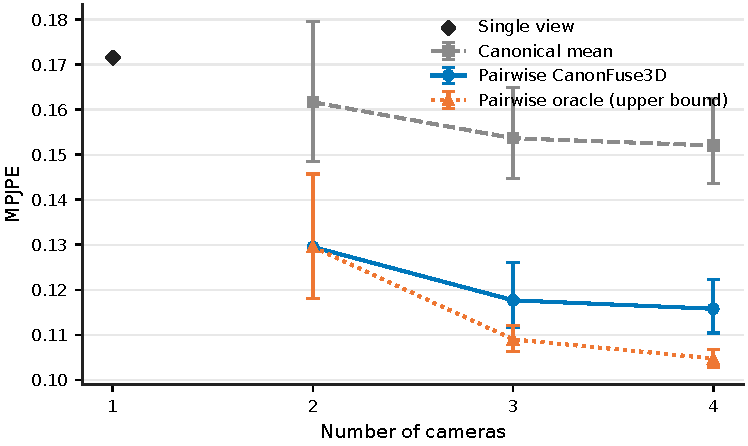
\includegraphics[width=0.72\linewidth]{figures/extension/nview_scaling.pdf}
\caption{N-view scaling under frozen pairwise CanonFuse3D composition. Error bars show paired-group bootstrap 95\% confidence intervals. The oracle is an upper bound.}
\label{fig:nview_scaling}
\end{figure}
}{%
\paragraph{Pending result} The N-view table and figure will be inserted only after the strict common-frame filter and the complete N=1--4 result matrix pass the artifact validator.
}

\FloatBarrier
\subsection{Automatic synchronization diagnostic}

\IfFileExists{tables/temporal_alignment.tex}{%
Figure~\ref{fig:temporal_alignment} compares uncorrected, automatically corrected, and oracle streams across the eleven injected offsets (exact errors, lag accuracy, and activation rates in Supplementary Table~\ref{S-tab:temporal_alignment}); the confidence threshold (0.09296) was fixed on validation data. The result is directionally asymmetric. Automatic correction improves MPJPE for every tested positive lag, at \(+5\) frames from 0.1537 to 0.1506 against the 0.1488 oracle, and gives smaller improvements at \(\pm0.5\) frames, but it worsens every tested negative integer lead, at \(-5\) frames from 0.1484 to 0.1498. At zero offset, 41.5\% of samples activate a nonzero correction and MPJPE rises from 0.14879 to 0.14884; exact lag accuracy is only 13.2\% at \(+5\) frames. The descriptor is therefore a useful diagnostic that partially recovers positive delays, not a reliable bidirectional synchronization solution, and it is not used in the main comparison.
\begin{figure}[!htb]
\centering
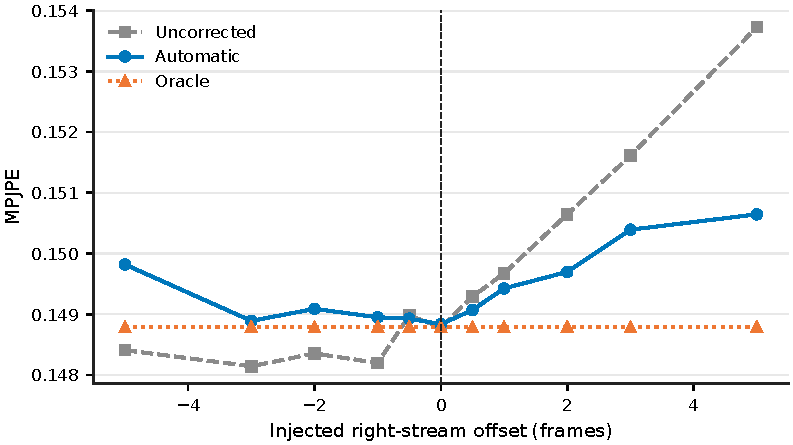
\includegraphics[width=0.72\linewidth]{figures/extension/temporal_alignment.pdf}
\caption{MPJPE under injected right-stream offsets on the fixed central 20-frame interval. Oracle restores the original unperturbed right stream; automatic correction uses the validation-calibrated confidence threshold.}
\label{fig:temporal_alignment}
\end{figure}
}{%
\paragraph{Pending result} Temporal-alignment results will be inserted only after all 33 offset-condition cells and the validation-threshold provenance pass validation.
}


\FloatBarrier
\subsection{Qualitative evaluation}

\begin{figure}[!htb]
\centering
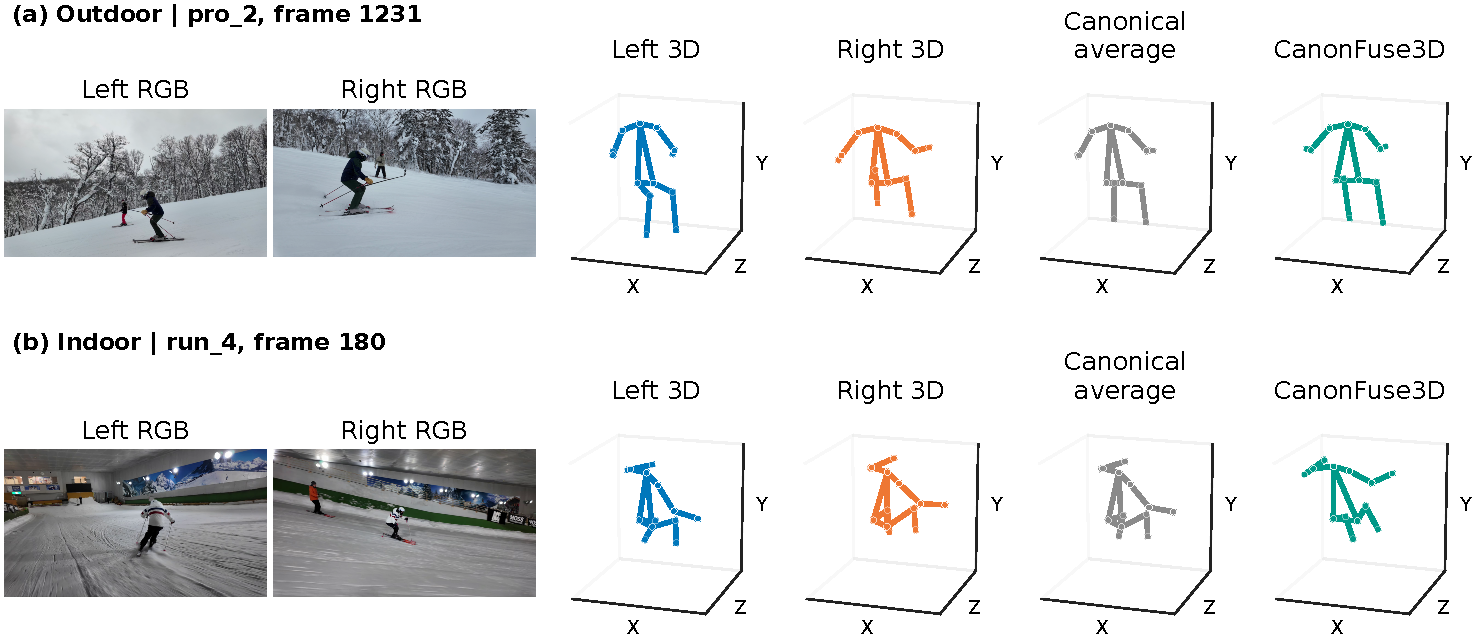
\includegraphics[width=0.98\textwidth]{figures/journal/realworld_qualitative_refresh.pdf}
\caption{Qualitative examples from author-collected (a) outdoor and (b) indoor recordings: the two input frames, the canonicalized single-view predictions, their average, and the frozen Unity-trained CanonFuse3D output at the midpoint of each clip (30-frame window, 13 joints, shared orientation and scale). No metric 3D reference exists for these clips.}
\label{fig:real_world_comparison}
\end{figure}

Figure~\ref{fig:real_world_comparison} illustrates deployment on two author-collected clips. Left- and right-view poses are estimated independently, and the frozen Unity-trained checkpoint processes a 30-frame window without camera calibration; fixed midpoint selection avoids choosing examples by apparent reconstruction quality, and the shared display scale preserves differences between the outputs. Without independent 3D ground truth, these examples demonstrate the inference workflow rather than an accuracy ranking, and similar errors in both upstream predictions can remain in the refined output.



\FloatBarrier
\section{Discussion}
\label{sec:discussion}

CanonFuse3D's advantage over non-learned pose-only controls supports learned refinement of complementary 3D streams, but the benchmark identifies no universal winner (Tables~\ref{tab:native_reference} and~\ref{tab:native_output_comparison}). Learned temporal methods trade position accuracy against smoothness, and geometric methods require additional 2D observations and calibration; the matched ablation attributes complementary position gains to gating and output residual correction, with an acceleration-error trade-off.

The useful deployment regime is approximately synchronized input with complementary evidence and an error distribution represented during training. Pairwise composition extends the frozen model to additional cameras without learning a joint multi-view representation; because its serial cost grows with the number of pairs, two views are the main accuracy--cost operating point in the evaluated implementation, although batching independent pairs could reduce latency without changing the pair count.

An estimator-agnostic architecture does not imply estimator-independent weights. Target-specific and mixed adaptation restore gains across the tested front ends, but recovery on a new estimator trades off against retention on SAM3D, so a new deployment should validate its upstream error distribution and, where needed, adapt the fusion model.

The RGB studies reveal limits that pose-only perturbations cannot expose. An unoccluded second view does not guarantee improvement over averaging under severe masking. Accurate supplied calibration favors learned geometric correction, whereas the larger tested calibration errors favor pose-only fusion on clean and moderately masked inputs (Section~\ref{subsec:matched_geometry}); position, aligned-shape, and acceleration errors need not favor the same method, and improved temporal agreement does not ensure accurate reconstruction, particularly when outputs collapse. The matched-image design characterizes sensitivity to supplied geometry, not the cost or accuracy of estimating that geometry during deployment.

\paragraph{Limitations}
All results come from one fixed partition and single training runs; bootstrap intervals describe resampling uncertainty conditional on the checkpoint, not variability across seeds or folds, and the 30-sequence Ski-PTZ-Pose index gives limited resolution between the learned models. Unity errors are measured against an avatar skeleton in dataset coordinates and Ski-PTZ-Pose errors against a constructed reference, so neither is independent metric 3D accuracy and no value should be relabeled in millimeters. The body reference is shared within each evaluation batch: regrouping can change the representation, missing reference landmarks can collapse other frames in the batch, and the severe-corruption results therefore characterize the coupled front-end, normalization, and prediction pipeline rather than the fusion network alone; small acceleration error for a collapsed output is not evidence of motion recovery. The gate is a learned reliability signal shaped by balance and entropy regularization, not calibrated uncertainty. Tolerance to small timing and rate perturbations does not extend to long delays, dropped frames, or independently varying frame rates; artificial patches on one frozen SAM3D front end do not establish robustness to natural occluders, weather, or motion blur, and the association between detection failure and fusion degradation is not causal; the alternative-front-end experiments lift ground-truth 2D tracks and so exclude image-detection noise. Broader validation requires external sports data, independent metric references, longer asynchronous sequences, and naturally occurring image degradation.

\section{Conclusion}
\label{sec:conclusion}

CanonFuse3D refines two approximately synchronized monocular 3D streams without images, 2D observations, or camera parameters at the fusion stage. It reduces canonical-space position error relative to averaging by 44.5\% on Unity and 48.6\% on Ski-PTZ-Pose. Learned temporal and geometry-assisted methods retain advantages on particular metrics or input regimes. Controlled studies delimit tolerance to camera separation, timing errors, and corruption: accurate supplied calibration can favor geometric correction, whereas larger tested calibration errors favor pose-only fusion on clean and moderately masked inputs. Severe image masking remains a failure regime, even with one unmasked view. Adaptation supports alternative front ends, and pairwise composition supports additional cameras, with two views offering the main evaluated accuracy--cost operating point. These fixed-partition, single-run results support deployment only after validating the upstream estimator and capture conditions. Cross-seed variability, independent physical 3D accuracy on real recordings, and broader real-world generalization remain open.

\section*{Funding}
This work was supported by the Japan Society for the Promotion of Science (JSPS) KAKENHI, Grant Numbers JP24K02978 and JP25K03146.

\section*{Acknowledgments}
We thank the dataset providers and the open-source research community for making this work possible. This research, in part, used computational resources of Pegasus provided by the Multidisciplinary Cooperative Research Program in the Center for Computational Sciences, University of Tsukuba. This work used computational resources of Pegasus provided by University of Tsukuba through the HPCI System Research Project (Project ID: hp260146).

\section*{Declaration of competing interest}
% CONFIRM: every author confirms nothing to declare; the same wording goes into the Elsevier declarations tool (.docx upload).
The authors declare that they have no known competing financial interests or personal relationships that could have appeared to influence the work reported in this paper.

\section*{CRediT authorship contribution statement}
% CONFIRM with all six authors. Funding acquisition follows KAKEN: JP25K03146 (PI Kitahara, co-I Xie) and JP24K02978 (co-I Kitahara).
\textbf{Kaixu Chen:} Conceptualization, Methodology, Software, Validation, Formal analysis, Investigation, Data curation, Writing -- original draft, Writing -- review \& editing, Visualization.
\textbf{Qingyu Wang:} Software, Investigation, Data curation, Validation.
\textbf{Chun Xie:} Methodology, Resources, Supervision, Funding acquisition, Writing -- review \& editing.
\textbf{Eiichi Naito:} Conceptualization, Resources, Writing -- review \& editing.
\textbf{Toshitaka Kimura:} Conceptualization, Resources, Writing -- review \& editing.
\textbf{Itaru Kitahara:} Conceptualization, Resources, Supervision, Project administration, Funding acquisition, Writing -- review \& editing.

\section*{Data and code availability}
% CONFIRM: release scope and timing of the Unity data and checkpoint (GitHub repository is already public; a DOI-minting archive such as Zenodo is recommended for the data).
The Ski-PTZ-Pose dataset is publicly available from the dataset provider~\cite{ski_poseptz_dataset}. The source code of CanonFuse3D, the training and evaluation scripts, the fixed train--validation--test indices, and the evaluation manifests recording checkpoint and front-end estimator hashes are available at \url{https://github.com/ChenKaiXuSan/skiing_dual2pose}. The Unity synthetic dataset and the frozen CanonFuse3D checkpoint used in all reported experiments will be deposited in a public repository with a persistent identifier upon publication. The author-collected indoor and outdoor recordings contain identifiable individuals and are not shared; they are used solely for qualitative illustration and contribute neither training samples nor quantitative measurements.

\section*{Ethics statement}
% CONFIRM: who appears in the author-collected clips, that written consent covers publication of the frames, and whether University of Tsukuba required an ethics review or an exemption.
The quantitative experiments use a synthetic dataset and the previously released Ski-PTZ-Pose dataset and involved no new data collection from human participants. The author-collected indoor and outdoor recordings used for qualitative illustration show adult volunteers from the authors' group who gave written informed consent to be recorded and to appear in the published figures. No other identifiable individuals are shown, and no personal data beyond the illustrated frames are released. The recordings were non-invasive observational video captures of consenting adults and did not require institutional ethics review under the guidelines of the University of Tsukuba.

% Journal rule: keep this exact section title, place it before the reference list, and use the template sentence.
% CONFIRM: tool names and scope. Elsevier only asks about the writing process; delete the section if no AI tool was used for writing.
\section*{Declaration of Generative AI and AI-assisted technologies in the writing process}
During the preparation of this work the authors used Claude (Anthropic) and OpenAI Codex to improve the readability and language of the manuscript. After using these tools, the authors reviewed and edited the content as needed and take full responsibility for the content of the publication.

\setlength{\bibsep}{4pt}
\bibliographystyle{elsarticle-num}
\bibliography{references}

\end{document}
